%% For double-blind review submission, w/o CCS and ACM Reference (max submission space)
\documentclass[10pt,conference]{ieeetran}%\settopmatter{printfolios=true,printccs=false,printacmref=false}

\usepackage{booktabs}   %% For formal tables:
                        %% http://ctan.org/pkg/booktabs
\usepackage{subcaption} %% For complex figures with subfigures/subcaptions
                        %% http://ctan.org/pkg/subcaption
\usepackage{amsmath,amsthm,amssymb}

\usepackage{xcolor,listings}

\usepackage{tikz}

\usepackage{array,multirow}

\usepackage{stmaryrd}

\usepackage[noadjust]{cite}

\theoremstyle{definition}
\newtheorem{definition}{Definition}

\newif\ifdraft \drafttrue
\newif\iftext \textfalse
\newif\iflater \latertrue
\newif\ifaftersubmission \aftersubmissionfalse

% !!! PLEASE DON'T CHANGE THESE !!! INSTEAD DEFINE YOUR OWN texdirectives.tex !!!
\makeatletter \@input{texdirectives} \makeatother

%\IEEEoverridecommandlockouts
% The preceding line is only needed to identify funding in the first footnote. If that is unneeded, please comment it out.
\usepackage{cite}
\usepackage{amsmath,amssymb,amsfonts}
\usepackage{algorithmic}
\usepackage{hyperref}
\usepackage{graphicx}
\usepackage{textcomp}
\usepackage[capitalize]{cleveref}
\usepackage[inline]{enumitem}

\usepackage{xcolor}
\newcommand{\bcp}[1]{\ifdraft\textcolor{violet}{{[BCP:~#1]}}\fi}
\newcommand{\leo}[1]{\ifdraft\textcolor{teal}{{[LEO:~#1]}}\fi}
\newcommand{\apt}[1]{\ifdraft\textcolor{blue}{{[APT:~#1]}}\fi}
\newcommand{\rb}[1]{\ifdraft\textcolor{orange}{{[RB:~#1]}}\fi}
\newcommand{\sna}[1]{\ifdraft\textcolor{green}{{[SNA:~#1]}}\fi}
\newcommand{\COQ}[1]{\ifdraft\textcolor{red}{{[COQ DIFFERENCE:~#1]}}\fi}

\usepackage{listings}


\usepackage{xspace}
\newcommand{\cn}{\ifdraft\textsuperscript{\textcolor{blue}{[citation needed]}}\xspace\fi}

\makeatletter
\begingroup
\lccode`\A=`\-
\lccode`\N=`\N
\lccode`\V=`\V
\lowercase{\endgroup\def\memory@noval{ANoValue-}}
\long\def\memory@fiBgb\fi#1#2{\fi}
\long\def\memory@fiTBb\fi#1#2#3{\fi#2}
\newcommand\memory@ifnovalF[1]%>>=
  {%
    \ifx\memory@noval#1%
      \memory@fiBgb
    \fi
    \@firstofone
  }%=<<
\newcommand\memory@ifnovalTF[1]%>>=
  {%
    \ifx\memory@noval#1%
      \memory@fiTBb
    \fi
    \@secondoftwo
  }%=<<
\newcommand\memory@Oarg[2]%>>=
  {%
    \@ifnextchar[{\memory@Oarg@{#2}}{#2{#1}}%
  }%=<<
\long\def\memory@Oarg@#1[#2]%>>=
  {%
    #1{#2}%
  }%=<<
\newcommand*\memory@oarg%>>=
  {%
    \memory@Oarg\memory@noval
  }%=<<
\newcommand*\memory@ifcoloropt%>>=
  {%
    \@ifnextchar[\memory@ifcoloropt@true\memory@ifcoloropt@false
  }%=<<
\long\def\memory@ifcoloropt@true#1\memory@noval#2#3%>>=
  {%
    #2%
  }%=<<
\long\def\memory@ifcoloropt@false#1\memory@noval#2#3%>>=
  {%
    #3%
  }%=<<
\newlength\memory@width
\newlength\memory@height
\setlength\memory@width{23pt}
\setlength\memory@height{14pt}
\newcount\memory@num
\newcommand*\memory@blocks[2]%>>=
  {%
    \memory@num#1\relax
    \fboxsep-\fboxrule
    \memory@ifcoloropt#2\memory@noval
      {\def\memory@color{\textcolor#2}}
      {\def\memory@color{\textcolor{#2}}}%
    \loop
    \ifnum\memory@num>0
      \fbox{\memory@color{\rule{\memory@width}{\memory@height}}}%
      \kern-\fboxrule
      \advance\memory@num\m@ne
    \repeat
  }%=<<
% memory:
%  [#1]: width
%   #2 : count
%  [#3]: height
%   #4 : colour
%  [#5]: label
\newcommand*\memory%>>=
  {%
    \begingroup
    \memory@oarg\memory@a
  }%=<<
\newcommand*\memory@a[2]%>>=
  {%
    % #1 width
    % #2 count
    \memory@ifnovalF{#1}{\memory@width#1\relax}%
    \memory@Oarg\memory@height{\memory@b{#2}}%
  }%=<<
\newcommand*\memory@b[3]%>>=
  {%
    % #1 count
    % #2 height
    % #3 colour
    \memory@ifnovalF{#2}{\memory@height#2\relax}%
    \memory@oarg{\memory@c{#1}{#3}}%
  }%=<<
\newcommand*\memory@c[3]%>>=
  {%
    % #1 count
    % #2 colour
    % #3 label
    \memory@ifnovalTF{#3}
      {\ensuremath{\memory@blocks{#1}{#2}}}
      {\ensuremath{\underbrace{\memory@blocks{#1}{#2}}_{\text{#3}}}}%
    \endgroup
  }%=<<
\makeatother

\newcommand{\judgment}[2]{
  {\centering
  \vspace{\abovedisplayskip}
  \begin{tabular}{c}
    #1 \\
    \hline
    #2
  \end{tabular}
   \vspace{\abovedisplayskip}\par}}

\newcommand{\judgmentbr}[4]{
  {\centering
  \vspace{\abovedisplayskip}
  \begin{tabular}{c}
    #1 \\
    #2 \\
    #3 \\
    \hline
    #4
  \end{tabular}
   \vspace{\abovedisplayskip}\par}}


\newcommand{\judgmenttwo}[3]{
  {\centering
  \vspace{\abovedisplayskip}
  \begin{tabular}{c c}
    #1 & #2 \\
    \hline
    \multicolumn{2}{c}{#3}
  \end{tabular}
  \vspace{\abovedisplayskip}\par}}

\newcommand{\judgmentthree}[4]{
  {\centering
  \vspace{\abovedisplayskip}
  \begin{tabular}{c c c}
    #1 & #2 & #3 \\
    \hline
    \multicolumn{3}{c}{#4}
  \end{tabular}
  \vspace{\abovedisplayskip}\par}}

% Notational conventions
\newcommand{\HIGHSEC}{\textsc{HC}}
\newcommand{\LOWSEC}{\textsc{LC}}
\newcommand{\HIGHINT}{\textsc{HI}}
\newcommand{\LOWINT}{\textsc{LI}}
\newcommand{\IDS}{{\mathcal{I}}}
\newcommand{\ID}{I}
\newcommand{\ME}{\textsc{S}}
\newcommand{\NOTME}{\textsc{O}}
\newcommand{\TRANS}{\ensuremath{-}}
\newcommand{\JAL}{\ensuremath{\mathit{JAL}}}
\newcommand{\ACCYES}{\ensuremath{A}}
\newcommand{\ACCNO}{\ensuremath{I}}
\newcommand{\ACCCODE}{\ensuremath{K}}
\newcommand{\CRCALL}{\ensuremath{\mathit{CALL}}}
\newcommand{\CRRET}{\ensuremath{\mathit{RETURN}}}
\newcommand{\CRBOT}{\ensuremath{\bot}}
\newcommand{\VIS}{\textsc{vis}}
\newcommand{\HID}{\textsc{hid}}
\newcommand{\word}{w}
\newcommand{\addr}{a}
\newcommand{\WORDS}{{\mathcal W}}
\newcommand{\reg}{r}
\newcommand{\REGS}{{\mathcal R}}
\newcommand{\mach}{m}
\newcommand{\machT}{M}
\newcommand{\MACHS}{{\mathcal M}}
\newcommand{\MPT}{\mathit{MP}}
\newcommand{\obs}{o}
\newcommand{\obsT}{O}
\newcommand{\OBSS}{\mathit{Obs}}
\newcommand{\PC}[1]{\PCname(#1)}
\newcommand{\PCname}{\textsc{pc}}
\newcommand{\SP}{\textsc{sp}}
\newcommand{\pol}{p}
\newcommand{\POLS}{\mathcal{P}}
\newcommand{\pinit}{pinit}
\newcommand{\prop}{S}
\newcommand{\contour}{C}
\newcommand{\CONTOURS}{{\mathcal C}}
\newcommand{\component}{k}
\newcommand{\COMPONENTS}{{\mathcal K}}
\newcommand{\trace}{T}
\newcommand{\observer}{O}
\newcommand{\stateobs}{\sigma}
\newcommand{\seq}[1]{\overline{#1}}
\newcommand{\SEQ}[1]{\overline{#1}}
\newcommand{\dstk}[1]{{#1}.\mbox{\it stack}}
\newcommand{\dpcd}[1]{{#1}.\mbox{\it PCdepth}}
\newcommand{\ddep}[2]{{#1}.\mbox{\it depth}({#2})}
\newcommand{\dinit}{\mbox{\it Dinit}}
\newcommand{\empstack}{\mbox{\it empty}}
\newcommand{\access}[2]{\mbox{\it accessible}_{#1}({#2})}
\newcommand{\norm}[1]{\lvert{#1}\rvert}
\newcommand{\MPS}{\mathit{MPState}}
\newcommand{\mpstate}[2]{(#1,#2)}
\newcommand{\mpostate}[3]{(#1,#2,#3)}
\newcommand{\mpstatename}{mp}
\newcommand{\callmap}{cm}
\newcommand{\CALLMAPS}{\mathit{CallMap}}
\newcommand{\ret}[1]{\mathit{justret}\ #1}
\newcommand{\nextPC}{next}
\newcommand{\base}{b}
\newcommand{\stepsto}{\Longrightarrow}
\newcommand{\stepstounder}[1]{\stackrel{\mbox{\tiny{$#1$}}}{\Longrightarrow}}
\newcommand{\stepstounderfull}{\stepstounder{\textsc{RISCV}}}
\newcommand{\manystepsto}{\stepsto^\star}
\newcommand{\obstrace}{\mathit{obstrace}}
\newcommand{\funid}{f}
\newcommand{\FUNIDS}{\mathcal{F}}
\newcommand{\retmap}{\mathit{rm}}
\newcommand{\RETMAPS}{\mathit{RetMap}}
\newcommand{\codemap}{\mathit{fm}}
\newcommand{\CODEMAPS}{\mathit{FuncMap}}
\newcommand{\entmap}{\mathit{em}}
\newcommand{\ENTMAPS}{\mathit{EntryMap}}
\newcommand{\PUT}{\mathit{Until}}
\newcommand{\Trace}{T}
\newcommand{\traceelem}{a}
\newcommand{\TRACEELEMS}{A}
\newcommand{\head}{\mathit{head}}
\newcommand{\last}{\mathit{last}}

\newcommand{\stepstoobs}[1]{\xrightarrow{#1}}
\newcommand{\polstep}{\rightharpoonup}
\newcommand{\stepstopol}[1]{\overset{#1}{\rightharpoonup}}
%\newcommand{\stepstopol}[1]{\overset{#1}{\rightharpoonup}_P}

\newcommand{\stepplus}{\Rightarrow}
\newcommand{\stepkappa}{\Rightarrow_\kappa}
\newcommand{\induced}[2]{(#1, #2)^*}
\newcommand{\flows}{\sqsubseteq}
\newcommand{\flowsstrict}{\sqsubset}
\newcommand{\initmach}{\MACHS_{\mathit{init}}}
\newcommand{\initcontour}{\CONTOURS_{\mathit{init}}}
\newcommand{\closure}[1]{\textit{Close}#1}
\newcommand{\variant}[2]{\textit{Vars}(#1, #2)}
\newcommand{\isinf}{\mathit{inf}}

\newcommand{\Last}[1]{\mathit{Last}(#1)}

\newcommand{\HALT}{\textsc{HALT}}

\newcommand{\underscore}{\mbox{\_}}

\newcommand{\propdef}[1]{\text{\sc #1}}

\newcommand{\TRACE}[1]{\mathit{Trace}~(#1)}
\newcommand{\MTRACE}{\TRACE{\MACHS}}
\newcommand{\MOTRACE}{\TRACE{\MACHS \times \OBSS}}
\newcommand{\MPOTRACE}{\TRACE{\MACHS \times \POLS \times \OBSS}}


\makeatletter
\newcommand{\linebreakand}{%
  \end{@IEEEauthorhalign}
  \hfill\mbox{}\par
  \mbox{}\hfill\begin{@IEEEauthorhalign}
}
\makeatother

\begin{document}

%% Title information
\title{Formalizing Stack Safety as a Security Property}

\author{
  \IEEEauthorblockN{
    Sean Noble Anderson
  }
  \IEEEauthorblockA{
    Portland State University\\
    ander28@pdx.edu\\
  }
  \and
  \IEEEauthorblockN{
    Leonidas Lampropoulos
  }
  \IEEEauthorblockA{
    University of Maryland, College Park\\
    leonidas@umd.edu\\
  }
  \and
  \IEEEauthorblockN{
    Roberto Blanco
  }
  \IEEEauthorblockA{
    Max Planck Institute for Security and Privacy\\
    roberto.blanco@mpi-sp.org\\
  }
  \linebreakand
  \IEEEauthorblockN{
    Benjamin C. Pierce
  }
  \IEEEauthorblockA{
    University of Pennsylvania\\
    bcpierce@cis.upenn.edu\\
  }
  \and
  \IEEEauthorblockN{
    Andrew Tolmach
  }
  \IEEEauthorblockA{
    Portland State University\\
    tolmach@pdx.edu\\
  }
}



%% Keywords
%% comma separated list
\ifcameraready
\keywords{Stack Safety, Micro-Policies}  %% \keywords are mandatory in final camera-ready submission
\fi

\maketitle

\begin{abstract}

``Stack safety'' is a term associated with a
variety of compiler, run-time, and hardware mechanisms for protecting stack
memory. But unlike heap memory, the stack does not correspond to any single
high-level language concept. The result is that
these mechanisms typically lack precise specifications,
relying instead on informal descriptions and examples of the bad
behaviors that they prevent. Such a specification is especially desirable
for an unusual enforcement mechanism, like the ``lazy'' stack safety
micro-policies proposed by Roessler and DeHon~\cite{DBLP:conf/sp/RoesslerD18}.

We propose a formal characterization of ``observable'' stack safety based on
concepts from language-based security. Stack safety is a
combination of an integrity property (``the private
state in each caller's stack frame is held invariant by the callee'')
and confidentiality properties (``the caller's and callee's behavior are
insensitive to one another's private state,''), both compatible with lazy tagging, as well as
control-flow property.

The stack governs a large number of language features that are often excluded
from discussion of stack safety. Our stack safety property targets a system with
both caller- and callee-saved registers, coroutines, arguments passed on the stack,
exceptions, [tail call elimination, heaps, and concurrency.]

We use these properties to validate Roessler and DeHon's micro-policies
via property-based random testing. Our testing successfully detects violations
in several broken variants, including Roessler and DeHon's original lazy policy.

\end{abstract}

\newcommand{\paragraphx}[1]{\emph{#1.}}

\section{Introduction}

The call stack is a perennial target for low-level attacks, leading to a
range of dire consequences, from leakage or corruption of private stack data
to control-flow hijacking. To foil such attacks, a profusion of
software and hardware protections have been proposed,
%
including stack canaries~\cite{Cowan+98},
bounds checking~\cite{NagarakatteZMZ09,NagarakatteZMZ10,DeviettiBMZ08},
split stacks~\cite{Kuznetsov+14},
shadow stacks~\cite{Dang+15,Shanbhogue+19},
capabilities~\cite{Woodruff+14,Chisnall+15,SkorstengaardLocal,SkorstengaardSTKJFP,Georges+21},
and hardware tagging~\cite{DBLP:conf/sp/RoesslerD18}.
  \ifaftersubmission\apt{Mostly from
  nick; there could be more}\bcp{Yes, going back to MIT days---we should
  include several more of these, if only to give readers the impression that
this is a well-studied mechanism (so formalizing its protections is
useful).}
\fi

The protections offered by such mechanisms are commonly described in terms
of concrete examples of attacks that they can prevent---corruption of return
addresses, buffer overflows, use of uninitialized variables, etc.---leaving
a more abstract characterization to the reader's intuition.  But these
mechanisms can be quite intricate, and the behaviors they aim to prevent are
subtle and varied. It can be hard to guess, based only on informal
intuitions, whether a given mechanism actually blocks all potential
attacks---or, conversely, whether it is overly conservative and disallows
system behaviors that are actually safe.
To settle such questions with confidence,
we need a precise, generic, and formal specification for stack
safety, as a basis both for comparing the security claims of different
enforcement techniques and for validating that these claims
are met by particular implementations. With the notable exception of the model used
in Skorstengaard et al.'s StkTokens work~\cite{SkorstengaardSTKJFP}, which we
discuss in Section \ref{sec:relwork}, there is a dearth of such properties in
the literature.

We propose a novel characterization of stack safety using the tools of language-based
security~\cite{sabelfeld2003language}, decomposing stack safety into
the {\em integrity} and {\em confidentiality} of the caller’s local state
during the callee's execution, and the confidentiality of the calle's local state
afterward, as well as the control flow protection of {\em well-bracketed control
  flow (WBCF)}~\cite{SkorstengaardSTKJFP}. We extend WBCF to a setting with exceptions,
in which there may be multiple points at which a callee can ``return.''

A key technical novelty in these definitions,
compared to standard formulations of confidentiality and integrity from the
security literature, is that they
are ``nested'': {\em each} caller is guaranteed protection from its
immediate callees (which, in turn, need protection from their immediate
callees, etc.).
Caller confidentiality is especially interesting. It is based on a traditional
notion of noninterference, but whereas ordinary noninterference
is an end-to-end hyper-property on whole program runs, caller
confidentiality is a nested form of noninterference that applies to
part of a run, requiring that the callee’s behavior is
invariant under hypothetical scrambling of the caller’s stack
but allowing the caller to access its own data upon return.

Our threat model is very strong, allowing the attacker
to execute arbitrary code, including attempting to smash
the stack to disrupt the program’s control flow. Our stack safety
properties demand that, even in the presence of such attackers, confidentiality
and integrity still apply.
%

For confidentiality and integrity, our properties are {\em observational},
meaning that they are only concerned with the observable behavior of the system.
A function activation might read from and write to other activations' data
without violating an observational property, as long as such reads and writes do not
affect the observable behavior of the
system. This permissiveness enables our properties to handle lazy enforcement mechanisms.

To demonstrate the utility of our formal characterization, we use these
properties to validate and improve an existing enforcement mechanism, the
{\em stack safety micro-policies} of Roessler and DeHon~\cite{DBLP:conf/sp/RoesslerD18}, re-implemented
in the Coq proof assistant on top of a RISC-V specification.  We
use QuickChick~\cite{Denes:VSL2014,Pierce:SF4}, a property-based testing
tool for Coq, to generate random programs and check
that Roessler and DeHon's micro-policies correctly abort the ones that
attempt to violate one of our properties. Furthermore, we
%
check that the testing framework is able to generate counterexamples
that violate our properties but are \emph{not} halted by incorrect
enforcement variants---both variants that we accidentally created
during our re-implementation of the micro-policy and ones that we
intentionally crafted to be broken in order to increase our confidence
in testing and the enforcement mechanism itself.

We find that Roessler and DeHon's {\em Depth Isolation} micro-policy, in
which memory within each stack frame is tagged with the depth of
the function activation that owns the frame and access is
permitted only when an activation at that depth is currently executing, validates our
stepwise properties. On the other hand, our testing reveals that \emph{Lazy Tagging and Clearing}
violates the temporal aspect of confidentiality in
cases where data can leak across repeated calls to the same callee,
and also violates integrity if the leak uses the caller's frame. We
propose a variant of {\em Lazy Tagging and Clearing} that testably enforces
confidentiality, albeit at some performance cost.

In sum, we offer the following contributions:

\begin{itemize}
\item We formalize permissive stack confidentiality and integrity and integrity properties.
  Both are parameterized over a notion of external
  observation, and are violated only if accessing secrets or overwriting
  data causes a visible change in the system behavior %(\cref{sec:lazy}).
\item We apply these definitions to a complex system with features such as argument passing
  on the stack, callee-saves registers, exceptions, and a simple coroutine system% (\cref{sec:ext}).
\item We use property-based random testing to validate the relationship between
  our properties and micro-policies %(\cref{sec:testing})
\end{itemize}
%\Cref{sec:relwork,sec:future} discuss related and future work.

Our artifact contains Coq formalizations of our properties for illustrative purposes
as well as the testing implementation.

\section{Machine Model and Security Semantics}

  We state our properties in terms of a generic machine, making minimal assumptions
  on the machine architecture and the nature of its built-in safety enforcement mechanisms
  (if any).  Our machine model is meant to be a faithful description of the hardware,
  with a semantics that covers both ordinary instruction behavior and the behavior of
  any tags, capabilities, etc. that the machine might support. 
  This semantics is intentionally \emph{not} ``safe-by-construction;'' it gives
  no guarantee that the enforcement hardware is being used correctly to achieve desired
  security properties. 

  On top of this machine model, we layer a {\it security semantics}, which extends the
  underlying machine with additional context about the identity of current and pending
  functions (which act as security principals) and about the registers and memory they require
  to be secure. This added context is purely notional;
  it does not affect the real machine. The security context
  evolves dynamically through the execution of {\it security-relevant operations},
  which include events like calls, returns, and frame manipulations.
  Our security properties are phrased in terms of this context, often as predicates
  on future states, e.g. of the form ``when control returns to the current function...'',
  or relations on traces of future execution (hyper-properties).

  The security-relevant operations typically correspond to underling machine instructions,
  but the correspondence may not be obvious just be inspecting the machine code.
  For example, in the tagged RISC-V machine we use in our examples and tests,
  calls and returns are conventionally performed by {\tt jal} (``jump-and-link'')
  and {\tt jalr} (``jump-and-link-register'') instructions, respectively, but these
  instructions might also be used for other things. We therefore assume that there
  is some external mechanism for distinguishing which instructions are security-relevant;
  the most obvious technique is to add optional labels to instructions, and that is 
  what we do in this paper, but the theory does not depend on this choice. 

  Our security semantics has similarities to the overlay semantics that have been proposed
  to characterize stack safety in the past~\cite{SkorstengaardSTK}, but, like the basic machine
  semantics, it is not safe-by-construction. Rather, it gives us a means to \emph{define}
  the security properties that a correct enforcement scheme should implement, using
  some combination of hardware and software.
  
In the next section, we give a detailed example of a security semantics for a simple setting
in which our security-relevant operations are restricted to making calls and returns, and allocating
private memory within the current function activation. In later sections, we extend this model
to the full system that we test, which features:
\begin{itemize}
\item Function calls and returns, with caller- and callee-saved registers
\item Allocation of strictly private and strictly public regions on the stack
\item Arguments spilled onto the stack and/or passed by reference
\item Exceptions
\item Tail-call Elimination
\end{itemize}

Finally, we give a property definition for stack safety in which (some) stack-allocated
objects are governed by a provenance-based capability system, accessible only to those
functions which have received a valid pointer to them.

%In section (TBD) we discuss the extension of this model into a simple concurrency setup.

\paragraph*{Threat Model}

We must trust that our method of distinguishing security-relevant operations is accurate; if it
involves labels placed on code by a compiler, that means trusting that the compiler placed
those labels correctly. If operations occur that are not recognized, those operations
might not be guaranteed to protect their principals---for instance, an unlabeled call
might not protect the caller's data from the callee. On the flip side, applying an incorrect
label most likely means that the property becomes too strong to be enforced.

Otherwise, we do not assume that the code adheres to any particular
calling convention or implements a source language construct.
In particular, while we are agnostic as to the source
language, we certainly aim to support C, and so any source function might contain undefined
behavior resulting in its compilation to arbitrary machine code. A given enforcement
mechanism may place additional constraints, particularly on the behavior of
call and return sequences.

In general, it is impossible to distinguish buggy source code from an attacker; in
our examples we will identify one function or another as an attacker, but we do not
require any static division between trusted and untrusted code, and we aim to protect
even buggy code.

This is a strong threat model, but hardware and timing attacks are out of scope,
and our properties are termination insensitive as a result of how failstops are
modelled (see ~\ref{??}).

\paragraph*{Limitations}

Our concurrency model is fairly
simplistic, assuming a fixed number of threads each with its own dedicated processor.
\sna{There is no concurrency in this document. Attempting to build it in from the beginning
  was rather complicated. The question is where to put that extra complexity? It's not difficult
  from a technical standpoint, subject to the one-thread-per-processor constraint.}
We model memory-safe stack objects, but not a heap. Regions outside of
stacks can be used however the compiler likes, including as a heap, but no protection is
built in and our properties assume that if a pointer to a stack object is stored there,
it is permanently compromised.

\subsection{The Basic Machine}

The building blocks of the machine are {\em words} and {\em registers}.
Words are ranged over by \(\word\) and, when used as addresses, \(\addr\),
and are drawn from the set \(\WORDS\).
Registers in the set \(\REGS\) are ranged over by \(\reg\), with the stack pointer
given the special name \(\SP\); 
some registers may be classified as caller-saved or callee-saved.
%
Along with the program counter, \(\PCname\), these are {\em state elements} \(\component\)
in the set \(\COMPONENTS ::= \PCname | \WORDS | \REGS\).

\begin{figure}
  \begin{tabular}{| l | l | l |}
    \hline
    Set / & Names & Purpose \\
    Class & & \\
    \hline
    \(\mathit{CLR}\) / & {\tt t0} -- {\tt t6} & Caller-saved temps \\
    \(\unsealed\) & {\tt a0} -- {\tt a1} & Caller-saved args / return vals \\
    & {\tt a2} -- {\tt a7} & Caller-saved args \\
    & {\tt ra} & Return Address \\
    \hline
    \(\mathit{CLE}\) / & {\tt s0} -- {\tt s11} & Callee-saved \\
    \(\sealed\) & {\tt sp} & Stack Pointer \\  
    \hline
    \(\mathit{PUBLIC}\) / & {\tt gp} & Global Pointer  \\
    \(\public\) & {\tt tp} & Thread Pointer \\
    \hline
  \end{tabular}
  \caption{RISC-V integer register set}
  \label{fig:RISCVregs}
\end{figure}

A {\em machine state} \(\mach\) is a map from elements to a set \(\mathcal{V}\) of
\emph{values}. Each value \(v\) contains a \emph{payload} word, written \(|v|\) (\(|\cdot|\).
The details of value structure depend on the specific machine being modelled;  
intuitively, the payload represents the part of the value that is relevant to
the behavior of the basic machine, while the rest of the value may contain
information relevant to a hardware enforcement mechanism (such as a tag).
We write \(\mach[\component]\) to denote the value at
\(\component\) of \(\mach\) and \(\mach[v]\) to denote the value at \(|v|\) if
defined.

{\em Events} are drawn from a set \(\OBSS\) and ranged over by \(\obs\), with a
special silent event \(\tau\).
The machine step function
\(\mach \xrightarrow{\overline{\psi},\obs} \mach' \in \MACHS \rightarrow
\MACHS \times \mathit{list} ~ \Psi \times \OBSS\)
is labeled by an ordered list of security-relevant operations, defined below,
and an event.

While some enforcement mechanisms may cause a machine to
failstop, we model this as the machine silently diverging by remaining in the
same state. We consider silently diverging traces to be indistinguishable
(from the point of view of an attacker) from traces that might eventually
produce output, an assumption that gives our properties the flavor of
{\it termination insensitivity}.

\subsection{Security-Relevant Operations, Principals, and Security State}

Security-relevant operations consist of calls, returns, and allocations.
Calls identify the address of the call's target,
and the argument registers. Allocations and deallocations are phrased in terms of a pair
of an offset from the stack pointer and a size. Returns don't require any additional information.
%
\begin{align*}
  \psi \in \Psi ::= & \mathbf{call} ~ \addr_{target} ~ \overline{\reg_{args}} & \\
  | & \mathbf{return} & \\
  | & \mathbf{alloc} ~ \mathit{off ~ sz} & \mathit{off, sz} \in \mathbb{N} \\
  | & \mathbf{dealloc} ~ \mathit{off ~ sz} & \mathit{off, sz} \in \mathbb{N} \\
\end{align*}
%
Security principals are function activations: at any given time, pending activations
have security requirements that are recorded in a call stack, and the current
activation tracks context information that will inform its requirements when
it makes a call. Each activation has a {\it view}
of the system that maps each state element to a {\it security class}:
it may be private to an inactive principal (\(\sealed\)),
in an allocated object that is accessible to the current principal (\(\object\)),
available to be allocated (\(\unsealed\)), or
always accessible (\(\public\)). The {\it initial view} \(V_0\) maps all stack locations to \(\unsealed\),
all other locations to \(\public\), and registers based on which set they
belong to: % (Figure \ref{fig:RISCVregs}):
\(\sealed\) for callee-saved, \(\unsealed\) for caller-saved, and \(\public\) otherwise.
%Elements of \(\mathcal{P}\),
%such as the program counter, are always \(\public\). Even if they might deserve their
%own protection, that protection is orthogonal to stack safety.

A {\it context} is a pair of the current activation's view and 
a list of views representing the call stack (pending inactive
principals), ranged over by \(\sigma\).  
%\[\context \in \CONTEXTS ::= \mathit{VIEW \times list ~ VIEW}\]
The initial context is \(\context_0 = (V_0, \emplist)\).

As the machine takes a step that executes a particular operation, it updates the
corresponding context, as described informally in the following section, and formally
in Section \ref{sec:props}.

%\section{Calls, Returns, and Private Allocations}
\section{Properties by Example}

In this section we consider a simple setting with calls, returns, and private allocations,
on a RISC-V machine with a PIPE tagging system. Here 
\(\mathcal{V} ::= \mathcal{W} \times \mathcal{T}\),
for some type \(\mathcal{T}\) of tags to be elaborated later, with \(|(w,t)| = w\).
Figure \ref{fig:RISCVregs} gives an example division of the RISC-V registers into
security classes. 
Figure \ref{fig:main} gives the C code and corresponding compiled RISC-V code
for a function {\tt main}. (Code is compiled using the standard RISC-V
calling conventions~\cite{??}; the stack grows towards lower addresses. We assume that
{\tt main} begins at address 0 and its callee {\tt f} at address 100.)

{\tt main} takes a secret as its argument and initializes a variable to contain
potentially sensitive data. We assume that the only observable events are stores
to a special address, called {\tt out}. 
{\tt main} calls another function {\tt f},
and afterward may decide to output its secret based on the contents of
its sensitive data. In this case, since {\tt sensitive} is initialized to 0,
it should not---instead it will output the results of {\tt f}.

\begin{figure}
  \begin{subfigure}{\columnwidth}
    {\tt
      volatile int out;
      
      void main(int secret) \{

      ~ ~ int sensitive = 0;

      ~ ~ int res = f();

      ~ ~ if (sensitive == 42) 

      ~ ~ ~ ~ out = secret;

      ~ ~ else 

      ~ ~ ~ ~ out = res;

      \}}
  \end{subfigure}
  \begin{subfigure}{\columnwidth}
    \begin{tabular}{r l | l}
      \labeledrow{0:}{addi sp,sp,-20}{\(\mathbf{alloc} ~ (-20,20)\)}
      \labeledrow{4:}{sd ra,12(sp)}{}
      \labeledrow{8:}{sw a1,8(sp)}{}
      \labeledrow{12:}{sw zero,4(sp)}{}
      \labeledrow{16:}{jal f,ra}{\(\mathbf{call} ~ \mathtt{f} ~ \emplist ~ \emplist\)}
      \labeledrow{20:}{sw a0,0(sp)}{}
      \labeledrow{24:}{lw a4,4(sp)}{}
      \labeledrow{28:}{li a5,42}{}
      \labeledrow{32:}{bne a4,a5,L1}{}
      \labeledrow{36:}{lw a0,8(sp)}{}
      \labeledrow{40:}{sw a0,out}{}
      \labeledrow{44:}{j L2:}{}
      \labeledrow{L1, 48:}{lw a0,0(sp)}{}
      \labeledrow{52:}{sw a0,out}{}
      \labeledrow{L2, 56:}{ld ra,12(sp)}{}
      \labeledrow{60:}{addi sp,sp,20}{\(\mathbf{dealloc} ~ (0,20)\)}
      \labeledrow{64:}{jalr ra}{\(\mathbf{return}\)}
    \end{tabular}
  \end{subfigure}
  \begin{subfigure}{\columnwidth}
    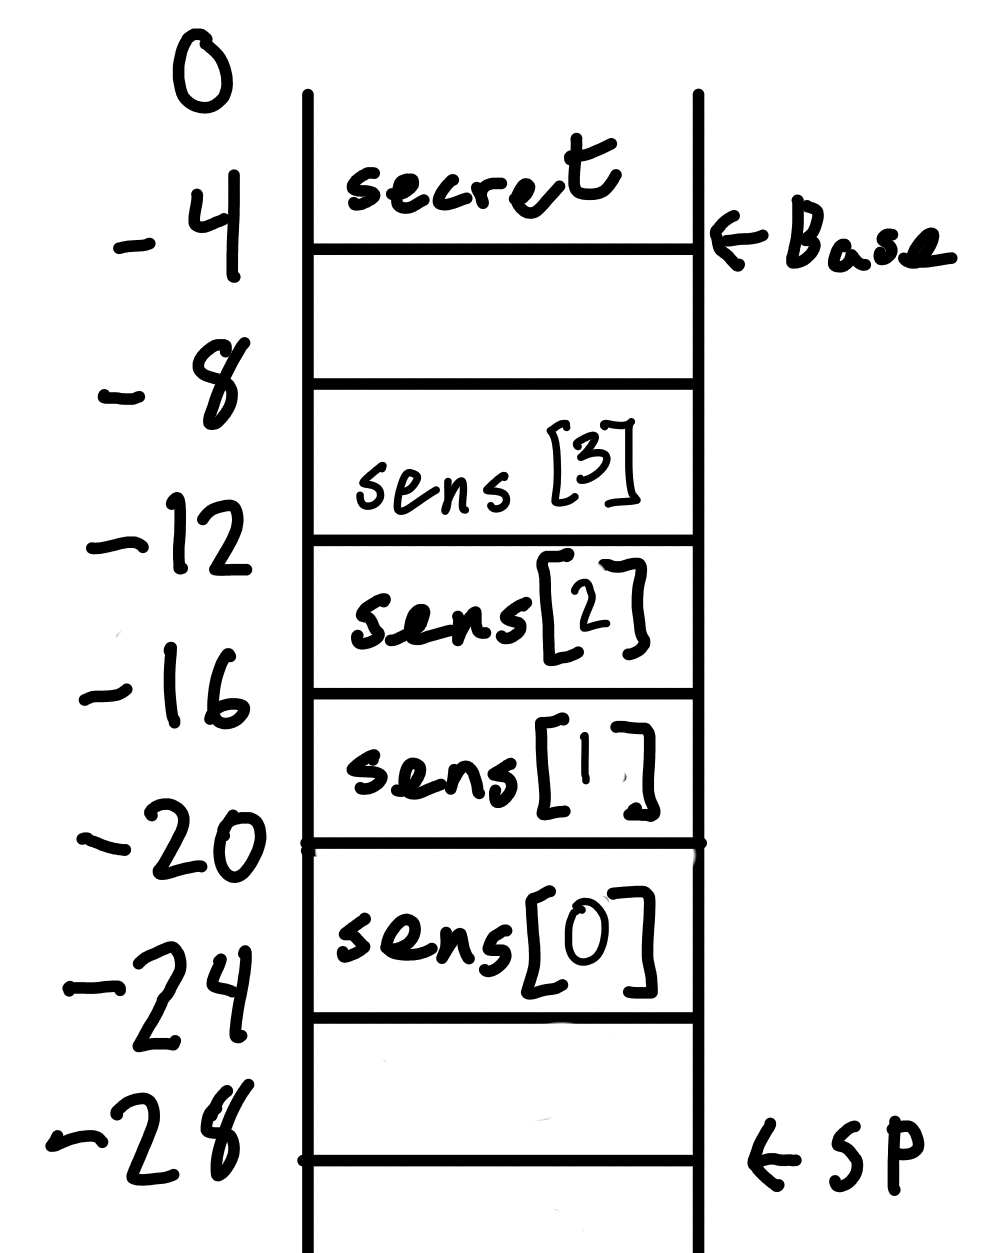
\includegraphics[width=\columnwidth]{stacklayout.png}
  \end{subfigure}

\caption{Example: Main}
\label{fig:main}
\end{figure}

Suppose that {\tt f} is not a (valid) C function at all, but an attacker seeking
to leak {\tt secret}! It might do so in a number of ways, shown as snippets of
assembly code in Figure \ref{fig:f}.\footnote{We arrange that all the snippets
have the same length just to simplify some later explanations.}
%
In Figure \ref{subfig:direct}, {\tt f} takes an offset from the stack
pointer, accesses {\tt secret}, and directly outputs it. But more
subtly, even if somehow prevented from outputting {\tt secret} directly, {\tt f}
can instead return that value so that {\tt main} stores it to {\tt out},
as in Figure \ref{subfig:indirect}.
%
Beyond simply reading {\tt secret}, the attacker might overwrite {\tt sensitive}
with 42, guaranteeing that {\tt main} publishes its own secret unintentionally
(Figure \ref{subfig:integrity})!
Attacks of this kind do not violate {\tt main}'s confidentiality, but its
{\it integrity}.
In Figure \ref{subfig:WBCF}, the attacker arranges to return to the
wrong instruction, thereby bypassing the check and publishing {\tt secret} regardless,
violating the program's {\it well-bracketed control flow} (WBCF.) Figure \ref{subfig:WBCF2}
shows another attack that violates WBCF, this time by returning to the correct
program counter but with the stack pointer offset.

\begin{figure}
  \begin{subfigure}[b]{\columnwidth}
    \vspace{\abovedisplayskip}
    \begin{tabular}{r l | l}
      \labeledrow{100:}{lw a4,8(sp)}{}
      \labeledrow{104:}{sw a4,out}{}
      \labeledrow{108:}{li a0,1}{}
      \labeledrow{112:}{jalr ra}{\(\mathbf{return}\)}
    \end{tabular}
    \caption{Leaking {\tt secret} directly}
    \label{subfig:direct}
  \end{subfigure}  
  \begin{subfigure}[b]{\columnwidth}
    \vspace{\abovedisplayskip}
    \begin{tabular}{r l | l}
      \labeledrow{100:}{lw a4,8(sp)}{}
      \labeledrow{104:}{mov a4,a0}{}
      \labeledrow{108:}{sw zero,-4(sp)}{}
      \labeledrow{112:}{jalr ra}{\(\mathbf{return}\)}
    \end{tabular}
    \caption{Leaking {\tt secret} indirectly}
    \label{subfig:indirect}
  \end{subfigure}  
  \begin{subfigure}[b]{\columnwidth}
    \vspace{\abovedisplayskip}
    \begin{tabular}{r l | l}
      \labeledrow{100:}{li a5,42}{}
      \labeledrow{104:}{sw a5,4(sp)}{}
      \labeledrow{108:}{li a0,1}{}
      \labeledrow{112:}{jalr ra}{\(\mathbf{return}\)}
    \end{tabular}
    \subcaption{Attacking {\tt sensitive}}
    \label{subfig:integrity}
  \end{subfigure}
  \begin{subfigure}[b]{\columnwidth}
    \vspace{\abovedisplayskip}
    \begin{tabular}{r l | l}
      \labeledrow{100:}{addi ra,ra,16}{}
      \labeledrow{104:}{nop}{}
      \labeledrow{108:}{nop}{}
      \labeledrow{112:}{jalr ra}{\(\mathbf{return}\)}
    \end{tabular}
    \subcaption{Attacking control flow}
    \label{subfig:WBCF}
  \end{subfigure}
  \begin{subfigure}[b]{\columnwidth}
    \vspace{\abovedisplayskip}
    \begin{tabular}{r l | l}
      \labeledrow{100:}{addi sp,sp,8}{}
      \labeledrow{104:}{nop}{}
      \labeledrow{108:}{nop}{}
      \labeledrow{112:}{jalr ra}{\(\mathbf{return}\)}
    \end{tabular}
    \subcaption{Relative address attack}
    \label{subfig:WBCF2}
  \end{subfigure}

  \caption{Assembly code for {\tt f} as an attacker}
  \label{fig:f}
\end{figure}

The security semantics for this program is based
on the security-relevant events noted in the right columns of Figures~\ref{fig:main}
and~\ref{fig:f}, namely execution of instructions that allocate or deallocate space,
make a call, or make a return.
Figure \ref{fig:exec1} shows how the corresponding security context
develops over the first few steps of the program. We assume execution begins
at the start of {\tt main} (\(\PCname = 0\)) and that the stack pointer is initially at
address 1000.
\(\xrightarrow{\overline{\psi}}\) transitions are numbered and
written \(\downarrow \overline{\psi}\) in this diagram; events are omitted.

Step 1 allocates a word each for {\tt secret}, {\tt sensitive}, and {\tt res}, as well
as two words for the return address. This will have the
effect of marking those bytes \(\object\), assuming they were previously
\(\unsealed\). (We use \(V\llbracket\cdot\rrbracket\) to denote updates to \(V\).)
%

\newcommand{\freebox}{\tikz \filldraw[fill=blue] (0,0) rectangle (10px,10px);}
\newcommand{\pubbox}{\tikz \filldraw[fill=lightgray] (0,0) rectangle (10px,10px);}
\newcommand{\objbox}{\tikz \filldraw[fill=yellow] (0,0) rectangle (10px,10px);}
\newcommand{\sealbox}{\tikz \filldraw[fill=red] (0,0) rectangle (10px,10px);}

\begin{figure*}
  \begin{tabular}{|r|r||l|r}
    \cline{1-3}
    \(\PCname\) & \(\SP\) & Context &
    \multirow{3}{*}{\(\underbrace{\dots \freebox \freebox \freebox \freebox \freebox
        \freebox \freebox \freebox \freebox \freebox}_\unsealed
      \! \underbrace{\stackrel{\stackrel{\SP}{\downarrow}}{\pubbox} \!\! \pubbox \pubbox \dots}_\public
      ~ \stackrel{\mathtt{a1}}{\pubbox} ~ \stackrel{\mathtt{a2}}{\freebox}
      ~ \stackrel{\mathtt{s0}}{\sealbox}
      \)} \\
    \cline{1-3}
    0 & 1000 & \(V_0, \emplist\)
    \\
    \cline{1-3}
    \multicolumn{3}{l}{\multirow{2}{*}{\(1 \Big\downarrow [\mathbf{alloc} ~ (-20,20)]\)}} & \\
    \multicolumn{3}{l}{} &
    \multirow{3}{*}{\(\underbrace{\dots \freebox \freebox \freebox \freebox \freebox}_\unsealed
      \! \underbrace{\stackrel{\stackrel{\SP}{\downarrow}}{\objbox} \!\! \objbox \objbox \objbox \objbox}_\object
      \! \underbrace{\pubbox \pubbox \pubbox \dots}_\public
      ~ \stackrel{\mathtt{a1}}{\pubbox} ~ \stackrel{\mathtt{a2}}{\freebox}
      ~ \stackrel{\mathtt{s0}}{\sealbox}
      \)}
    \\
    \cline{1-3}
    4 & 980 & \(V_1 = V_0 \llbracket 980..999 \mapsto \object\rrbracket, \emplist\) &
    \\
    \cline{1-3}
    \multicolumn{3}{l}{\multirow{2}{*}{2-4 \(\Big\downarrow \emplist\)}} \\ \multicolumn{3}{l}{} \\
    \cline{1-3}
    16 & 980 & \(V_1, \emplist\) & \\
    \cline{1-3}
    \multicolumn{3}{l}{\multirow{2}{*}{\(5 \Big\downarrow [\mathbf{call} ~ 100 ~ \emplist]\)}} & \\
    \multicolumn{3}{l}{} &
    \multirow{3}{*}{\(\underbrace{\dots \freebox \freebox \freebox \freebox \freebox}_\unsealed
      \! \underbrace{\stackrel{\stackrel{\SP}{\downarrow}}{\sealbox} \!\! \sealbox \sealbox \sealbox \sealbox}_\sealed
      \! \underbrace{\pubbox \pubbox \pubbox \dots}_\public
      ~ \stackrel{\mathtt{a1}}{\freebox} ~ \stackrel{\mathtt{a2}}{\freebox}
      ~ \stackrel{\mathtt{s0}}{\sealbox}
      \)}
    \\
    \cline{1-3}
    100 & 980 & \(V_2 = V_1 \llbracket 980..999 \mapsto \sealed, \mathtt{a0} \mapsto \unsealed\rrbracket,[V_1]\) & \\
    \cline{1-3}
    \multicolumn{3}{l}{\multirow{2}{*}{6-8 \(\Big\downarrow \emplist\)}} \\ \multicolumn{3}{l}{} \\
    \cline{1-3}
    112 & 980 & \(V_2,[V_1]\) \\
    \cline{1-3}
    \multicolumn{3}{l}{\multirow{2}{*}{\(9 \Big\downarrow [\mathbf{return}]\)}} & \\
    \multicolumn{3}{l}{} & \multirow{3}{*}{\(\underbrace{\dots \freebox \freebox \freebox \freebox \freebox}_\unsealed
      \! \underbrace{\stackrel{\stackrel{\SP}{\downarrow}}{\objbox} \!\! \objbox \objbox \objbox \objbox}_\object
      \! \underbrace{\pubbox \pubbox \pubbox \dots}_\public
      ~ \stackrel{\mathtt{a1}}{\pubbox} ~ \stackrel{\mathtt{a2}}{\freebox}
      ~ \stackrel{\mathtt{s0}}{\sealbox}
      \)}
    \\
    \cline{1-3}
    20 & 980  & \(V_1, \emplist\) &
    \\
    \cline{1-3}
    \multicolumn{2}{l}{} \\
  \end{tabular}
\caption{Execution up through the return from {\tt f}}
\label{fig:exec1}
\end{figure*}
%
At step 5, the formerly active principal's record is pushed onto the inactive list.
Its return target is the return address of the call, 
and the stack pointer target is the stack pointer at the moment of call.
The callee's view is updated from the caller's such that all \(\object\) locations
become \(\sealed\). (In more complex settings, objects that are intentionally passed
to the callee will not get sealed, but for now we assume no sharing of memory between activations.)
For registers, \(\overline{\reg_{args}}\) tells us which registers are used as arguments,
in this case just {\tt a0}. These are mapped to \(\public\), while any non-argument, caller-saved
registers remain mapped to \(\unsealed\). All callee-save registers remain \(\sealed\) for all calls.
At step 9, {\tt f} returns, and the topmost inactive view, that of {\tt main}, is restored.

We now show how this security semantics can be used define notions of confidentiality,
integrity, and correct control flow in such a way that many classes of
bad behavior, including the attacks in Figure~\ref{fig:f}, are 
are detected as security violations. 

\paragraph*{Well-bracketed Control Flow}

To begin with, what if {\tt f} returns to an unexpected place (i.e. \(\PCname \neq 20\) or
\(\SP \neq 980\))? We consider this to
violate well-bracketed control flow (WBCF). WBCF is a relationship between
call steps and their corresponding return steps: just after the return, the program
counter should be at the next instruction following the call,
and the stack pointer should be the same as it was before the call.

Consider the attack in Figure \ref{subfig:WBCF}: the attacker adds
16 to the return address and then returns, thus bypassing the {\tt if}-test in the code and outputting
{\tt secret}. Before the call, the program counter is 16 and the stack pointer is 980,
so we define a predicate on states that should hold just after the return:
\(\ret\ \mach \triangleq \mach[\PCname] = 20 \wedge \mach[\SP] = 980\).
%
We can identify the point just after the return (if a return occurs)
as the first state in which the pending call stack is smaller than it was
just after the call.
WBCF requires that if \(\mach\) is the state at that point, then \(\ret ~ \mach\) holds.
%For nested calls, where the pending stack is initially larger, the same principle
%applies: \(\ret ~ \mach\) must hold the next time the pending stack is the same size or smaller.

To see why WBCF also cares about the stack pointer, consider the attack in
Figure \ref{subfig:WBCF2}. Here the attacker returns with \(\SP' = 998\) instead of the
correct \(\SP = 980\). In this scenario, given the layout of {\tt main}'s frame 
\begin{tabular}{| l | l | l | l | l |}
  \multicolumn{1}{r}{\(\SP \downarrow\)} &
  \multicolumn{2}{r}{\(\SP' \downarrow\)} \\
  \hline
  res & sens & sec & ra & ra \\
  \hline
\end{tabular}

\vspace{\abovedisplayskip}

\noindent
{\tt main}'s attempt to read {\tt sensitive} will instead 
read part of the return address, and its attempt to output
{\tt res} will instead output {\tt secret}! Even absent other
kinds of data protection, the stack pointer {\it must} be restored
for the program to behave predictably.

In typical compiled code, WBCF is maintained by the compiler's call and return sequences.
As long as a function deallocates the same-sized frame that it allocates, and properly
saves and restores the return address, it should have WBCF---unless an error in the middle
subverts those sequences by overwriting one of the relevant elements, or by jumping into
the middle of the call or return sequence. We can therefore enforce WBCF by (1) ensuring that
these ``blessed'' call and return sequences execute in order and (2) permitting only blessed
sequences to write to \(\SP\), {\tt ra}, and the address in memory where {\tt ra} is stored.

To perform this enforcement using tags, we can take
\(\mathcal{T} ::= \mathit{gen} | \mathit{bseq} ~ n ~ m | \mathit{prot}\), named for general
execution, blessed sequence, and protected, respectively. Blessed sequences of length \(m\) are
tagged \(\mathit{bseq} ~ 1 ~ m\) through \(\mathit{bseq} ~ m ~ l\), and the micro-policy enforces
that they execute in order. The stack pointer and {\tt ra}
are tagged \(\mathit{prot}\). Only instructions tagged \(\mathit{bseq}\) may write to memory
or registers tagged \(\mathit{prot}\). Store instructions tagged \(\mathit{bseq}\) tag their
targets \(\mathit{prot}\).

\paragraph*{Stack Integrity}

Like WBCF, stack integrity defines a condition at the call that must hold upon
return. This time the condition applies to all of the memory that a function has
allocated. In Figure \ref{fig:exec1} we see the lifecycle of an allocated frame:
upon allocation, the view labels it \(\object\), and when a call is made, it instead
becomes \(\sealed\). Intuitively, the integrity of {\tt main}
is preserved if, when control returns to it, it can rely on any \(\sealed\) elements
to be identical to when it made the call.
%
Again, we need to know when a caller has been returned to,
and we use the same mechanism of checking the depth of the call stack.
%
In the case of the call from {\tt main} to {\tt f}, the \(\sealed\) elements are the
addresses 980 through 999 and callee-saved registers such as
the stack pointer. Note that callee-saved registers often change
during the call---but if the caller accesses them after the call, it should find them
restored to their prior value.

While it would be simple to define integrity as ``all sealed elements retain their
values after the call,'' this would be stricter than necessary for many purposes.
For example, it arguably doesn't matter if {\tt f} overwrites {\tt main}'s data provided
that {\tt main} never reads that corrupted data.
To illustrate, we can consider two integrity micro-policies: ``Depth Isolation'' and
``Lazy Tagging and Clearing.''

Depth Isolation tracks the depth of the current activation via a tag on the program counter.
Stack frames are initialized and cleared, by writing
to every address in them, so that during a call at depth \(d\), the current activation's
frame is tagged with \(d\). Loads and stores targeting addresses in frames failstop
if the program counter tag does not match the frame tag. In this setting, at depth \(d\),
all memory tagged with a depth less than \(d\) corresponds to \(\sealed\) memory,
and should be indeed be inaccessible. 

On the other hand, Lazy Tagging and Clearing skips the (inefficient)
initialization and clearing steps, and only updates tags when memory is written to.
It allows a callee to overwrite sealed memory, but that write tags the corrupted memory
with the callee's identity. Only if the corrupted memory's owner (or any other activation) tries
to read it will the micro-policy failstop.

Lazy Tagging and Clearing illustrates the value of ``extensional'' properties.
It is common to specify the behavior of a system, including security properties, in
terms of traces of observable events rather than details of the machine state.
Lazy enforcement works because the deferred check catches errors before they appear
in the trace. The nature of traces varies based on the properties of interest, but
given a particular model of observation, we can consider
corruption by {\tt f} acceptable as long as it does not affect {\tt main}'s observable behavior.

To characterize this situation in a property, we define a state element to be \emph{irrelevant}
if its value can be replaced with another value without changing the observable behavior
of the machine. This replacement value must respect any enforcement-relevant constraints on
values; in the tagged setting, we define two values as variants if they share the same tag
component. Then, for a set of elements \(\components\),
a pair of states \(\mach\) and \(\nach\) are {\em \(\components\)-variants} if
they agree on the value of every element not in \(\components\), and the values
in all elements are variants.

The elements of \(\components\) are \emph{irrelevant}
in \(\mach\) if every \(\components\)-variant state produces an equivalent observation trace
(see Section \ref{sec:events}); all other elements are \emph{relevant}.
We characterize \emph{observational integrity} as the property that
every relevant element that is \(\sealed\) under the callee's view is restored
to its original value at the return point.

\begin{figure}
  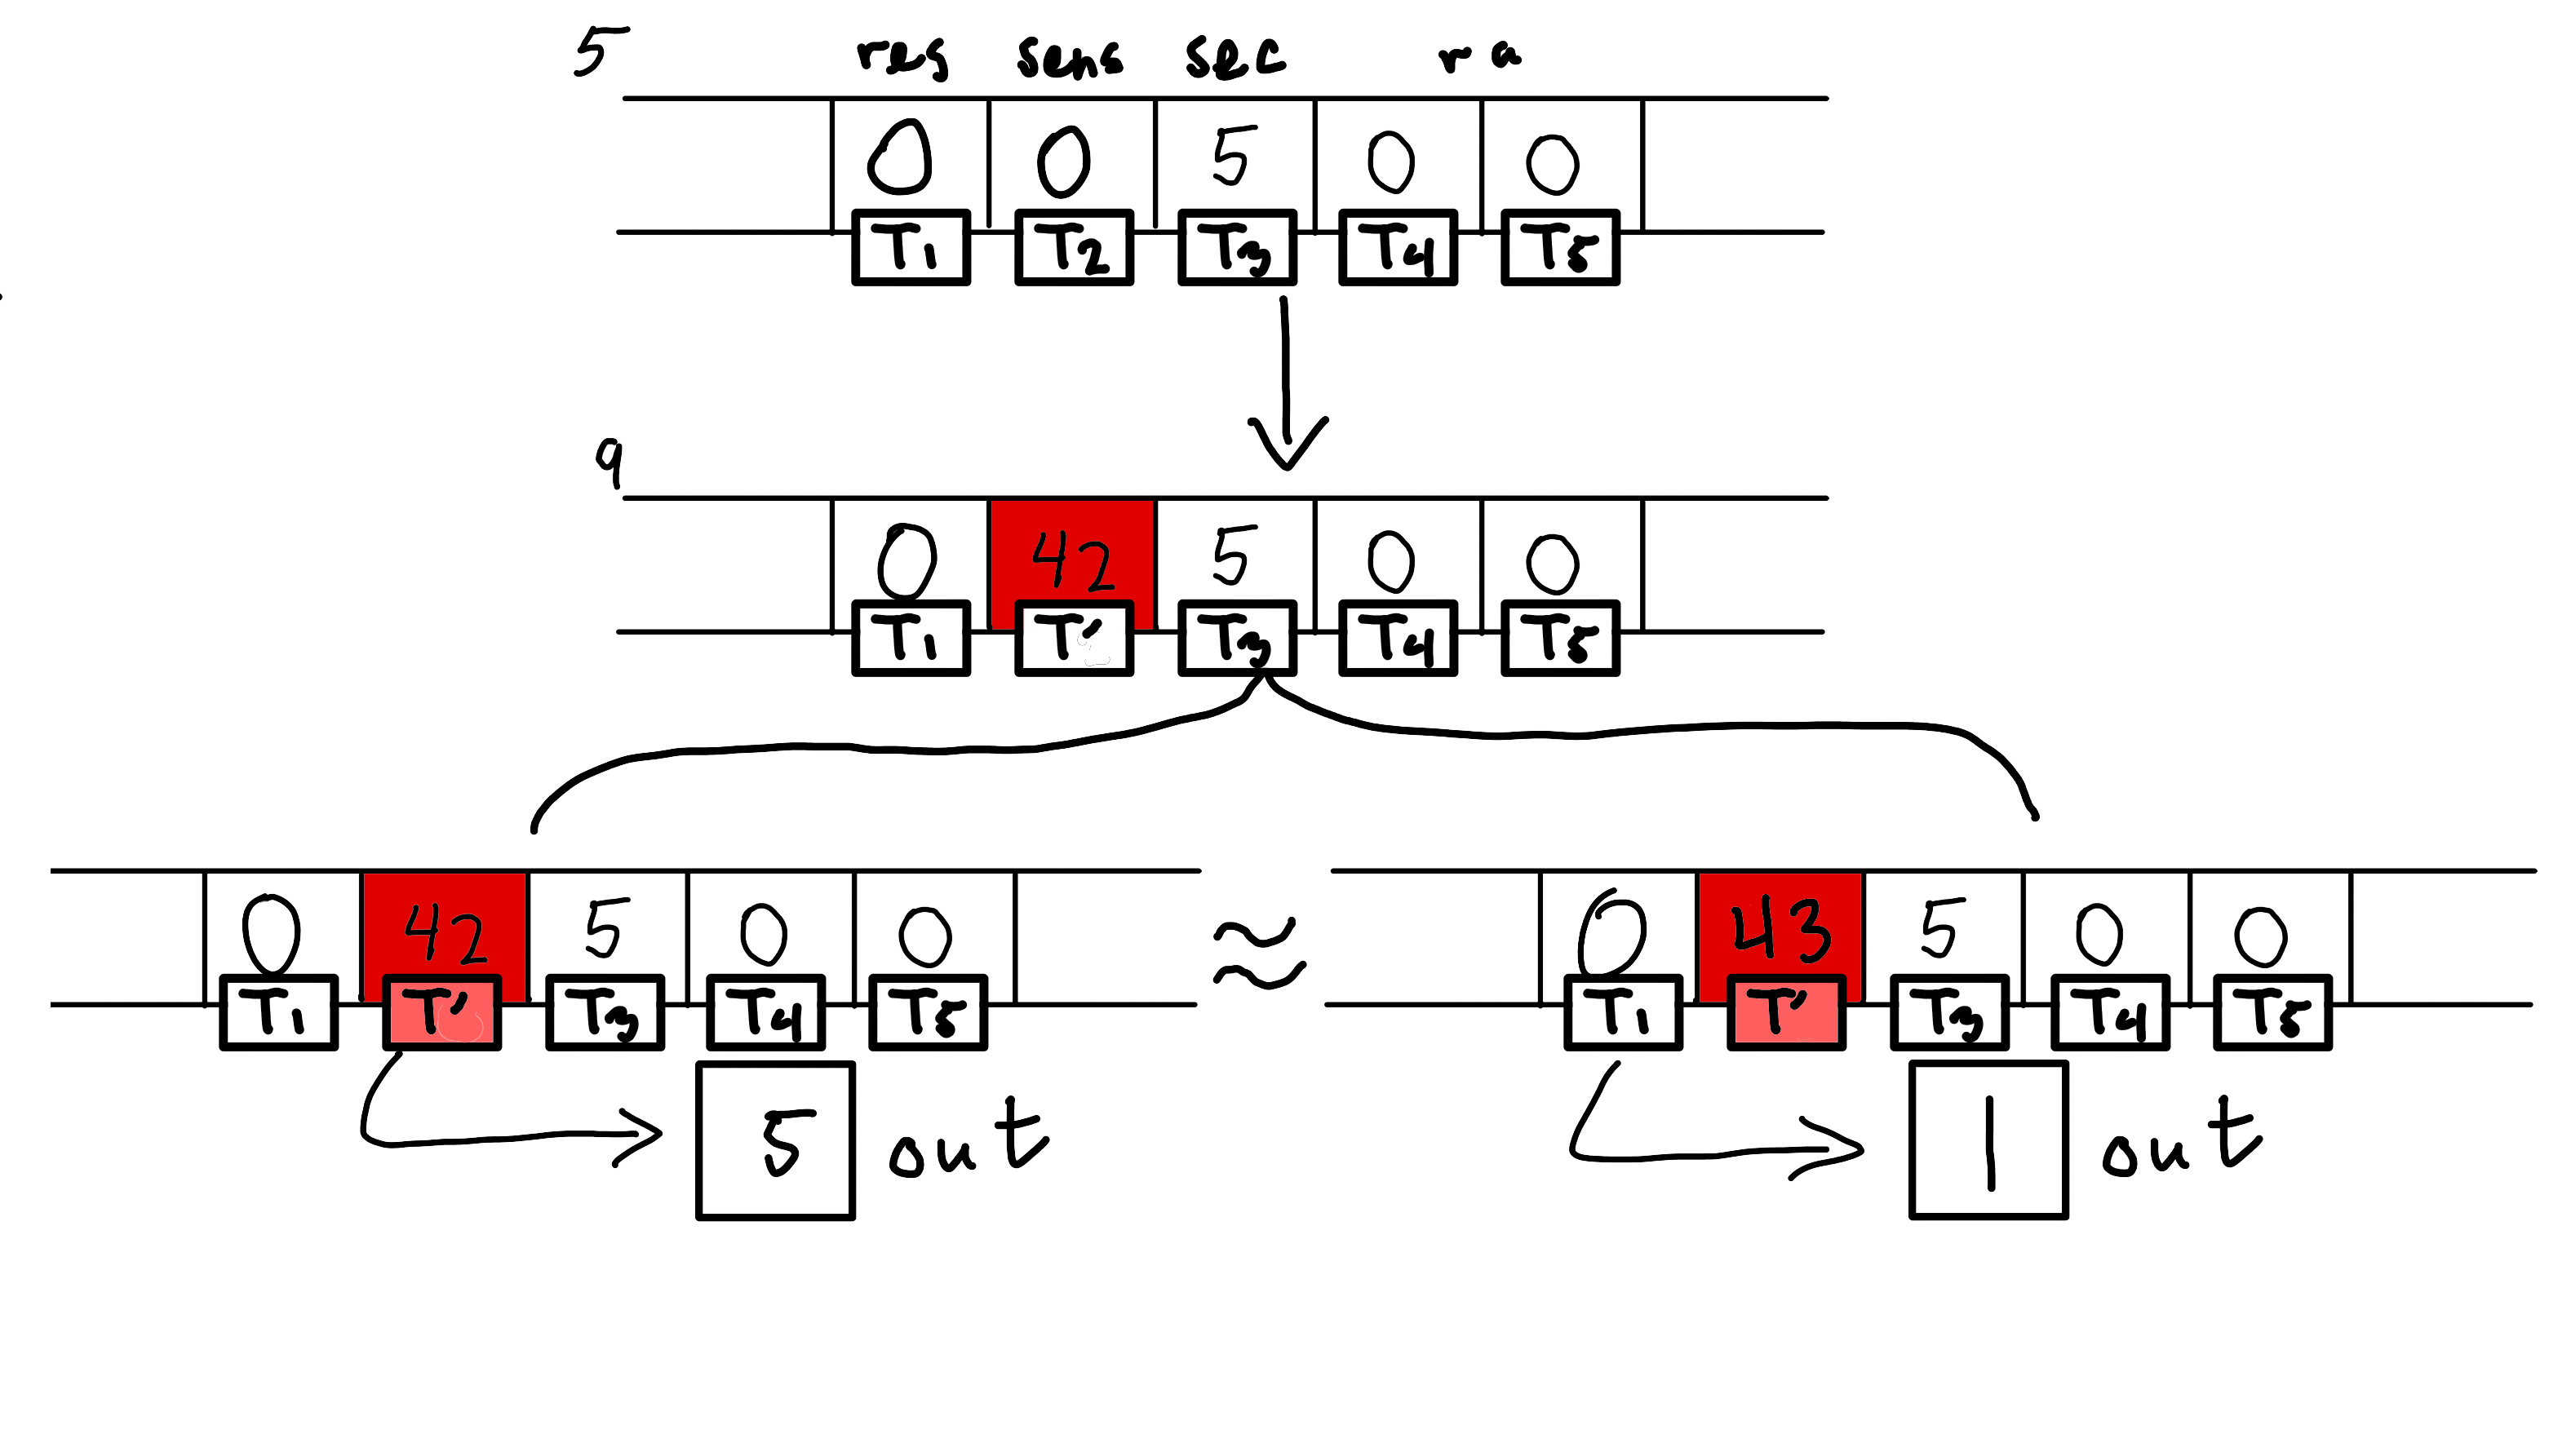
\includegraphics[width=\columnwidth]{variants.png}
  \caption{Integrity Violation}
  \label{fig:variant}
\end{figure}

In our example setting, the observation trace consists of the sequence of values written to {\tt out}.
The example in Figure \ref{subfig:integrity} modifies the value of {\tt sensitive},
which is \(\sealed\). Figure \ref{fig:variant} shows the state just after the call at step 5,
assuming that {\tt sec} is 5. Similar to WBCF, we will define
\(\intProp\) as a predicate on states that holds if
all relevant sealed addresses in \(\mach\) are the same as after step 5.
We once again require that \(\intProp\) hold on the state following the matching return, 
which is reached by step 9. Here {\tt sensitive} has obviously changed, but is it relevant?
Consider a variant state in which {\tt sensitive} has any other value, arbitrarily
choosing 43 (and keeping its tag, \(t_2'\), unchanged.) As execution continues after the return
from the original state, it passes the {\tt if}-test on {\tt sensitive}, whereas the execution
from the variant does not, resulting in differing outputs. Therefore {\tt sensitive} \emph{is} relevant,
so \(\intProp\) does not hold, and integrity has indeed been violated.

\paragraph*{Caller Confidentiality}

We treat confidentiality as a form of non-interference as well: the confidentiality of a caller
means that its callee's behavior is dependent only on publicly visible data,
not the caller's private state. This also requires that the callee initialize
memory before reading it.
As we saw in the examples, we must consider both the observable events
that the callee produces during the call and the changes that the callee makes to the state that might
affect the caller after the callee returns.

Consider the state \(\mach\) after step 5, whose context is \((V_2,\sigma)\), with the attacker from
Figure \ref{subfig:direct}. We take a variant state over the set of element(s) that are
\(\sealed\) or \(\unsealed\) in \(V_2\), which happens to be the entire stack (see
Figure \ref{fig:variant2}.) If we take a trace of execution from each state until it returns,
the traces may differ, in this case outputting 5 (the original value of {\tt secret}) and
4 (its value in the variant) respectively. This is a violation of
{\it internal confidentiality}.

\begin{figure}
  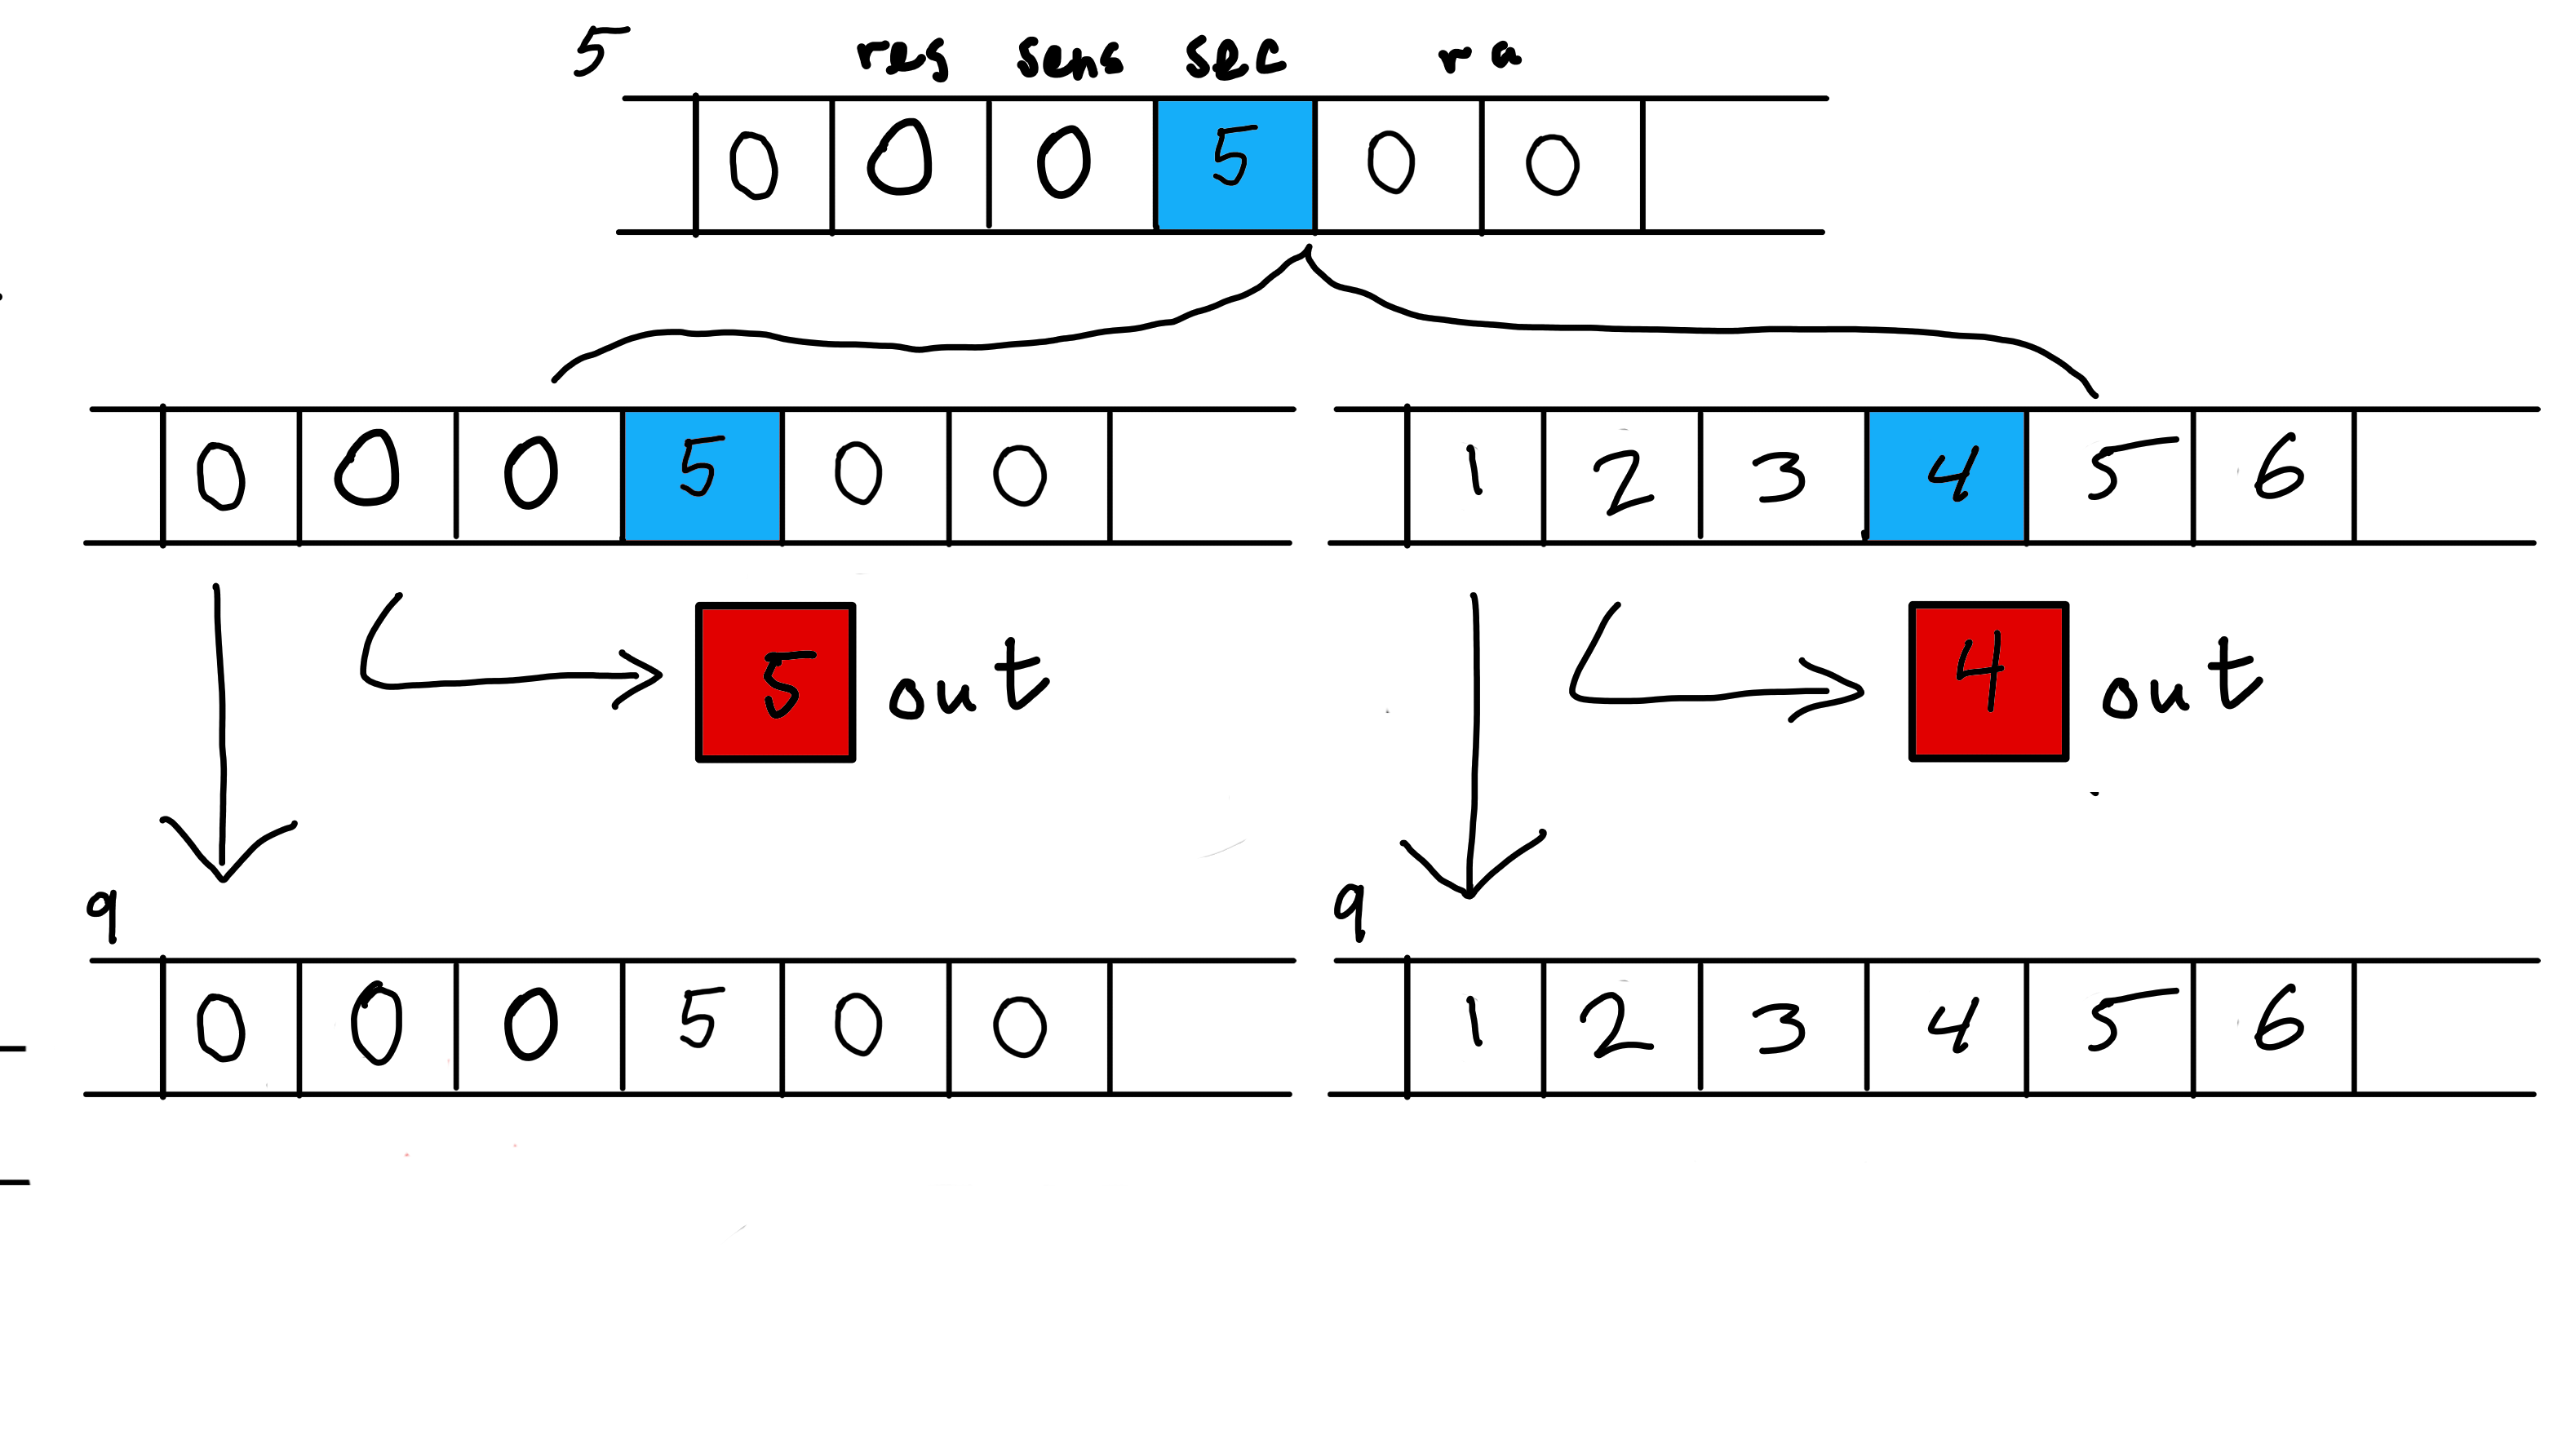
\includegraphics[width=\columnwidth]{variants2.png}
  \caption{Internal Confidentiality Violation}
  \label{fig:variant2}
\end{figure}

But, in Figure \ref{subfig:indirect}, we also saw an attacker that exfiltrated the secret
by reading it and then returning it, in a context where the caller would output the returned
value. Figure \ref{fig:variant3} shows the behavior of the same variants under this attacker,
but in this case, there is no output during the call. Instead the value of {\tt secret} is
extracted and placed in {\tt a0}, the return value register. We wish to identify this as
a confidentiality violation, again by considering variants of the \(\sealed\) and \(\unsealed\)
elements in \(V_2\), but capturing the required property is subtle.  

To illustrate the issues, note that {\tt f} has also stores a 0 below the stack pointer.
%
\begin{figure}
  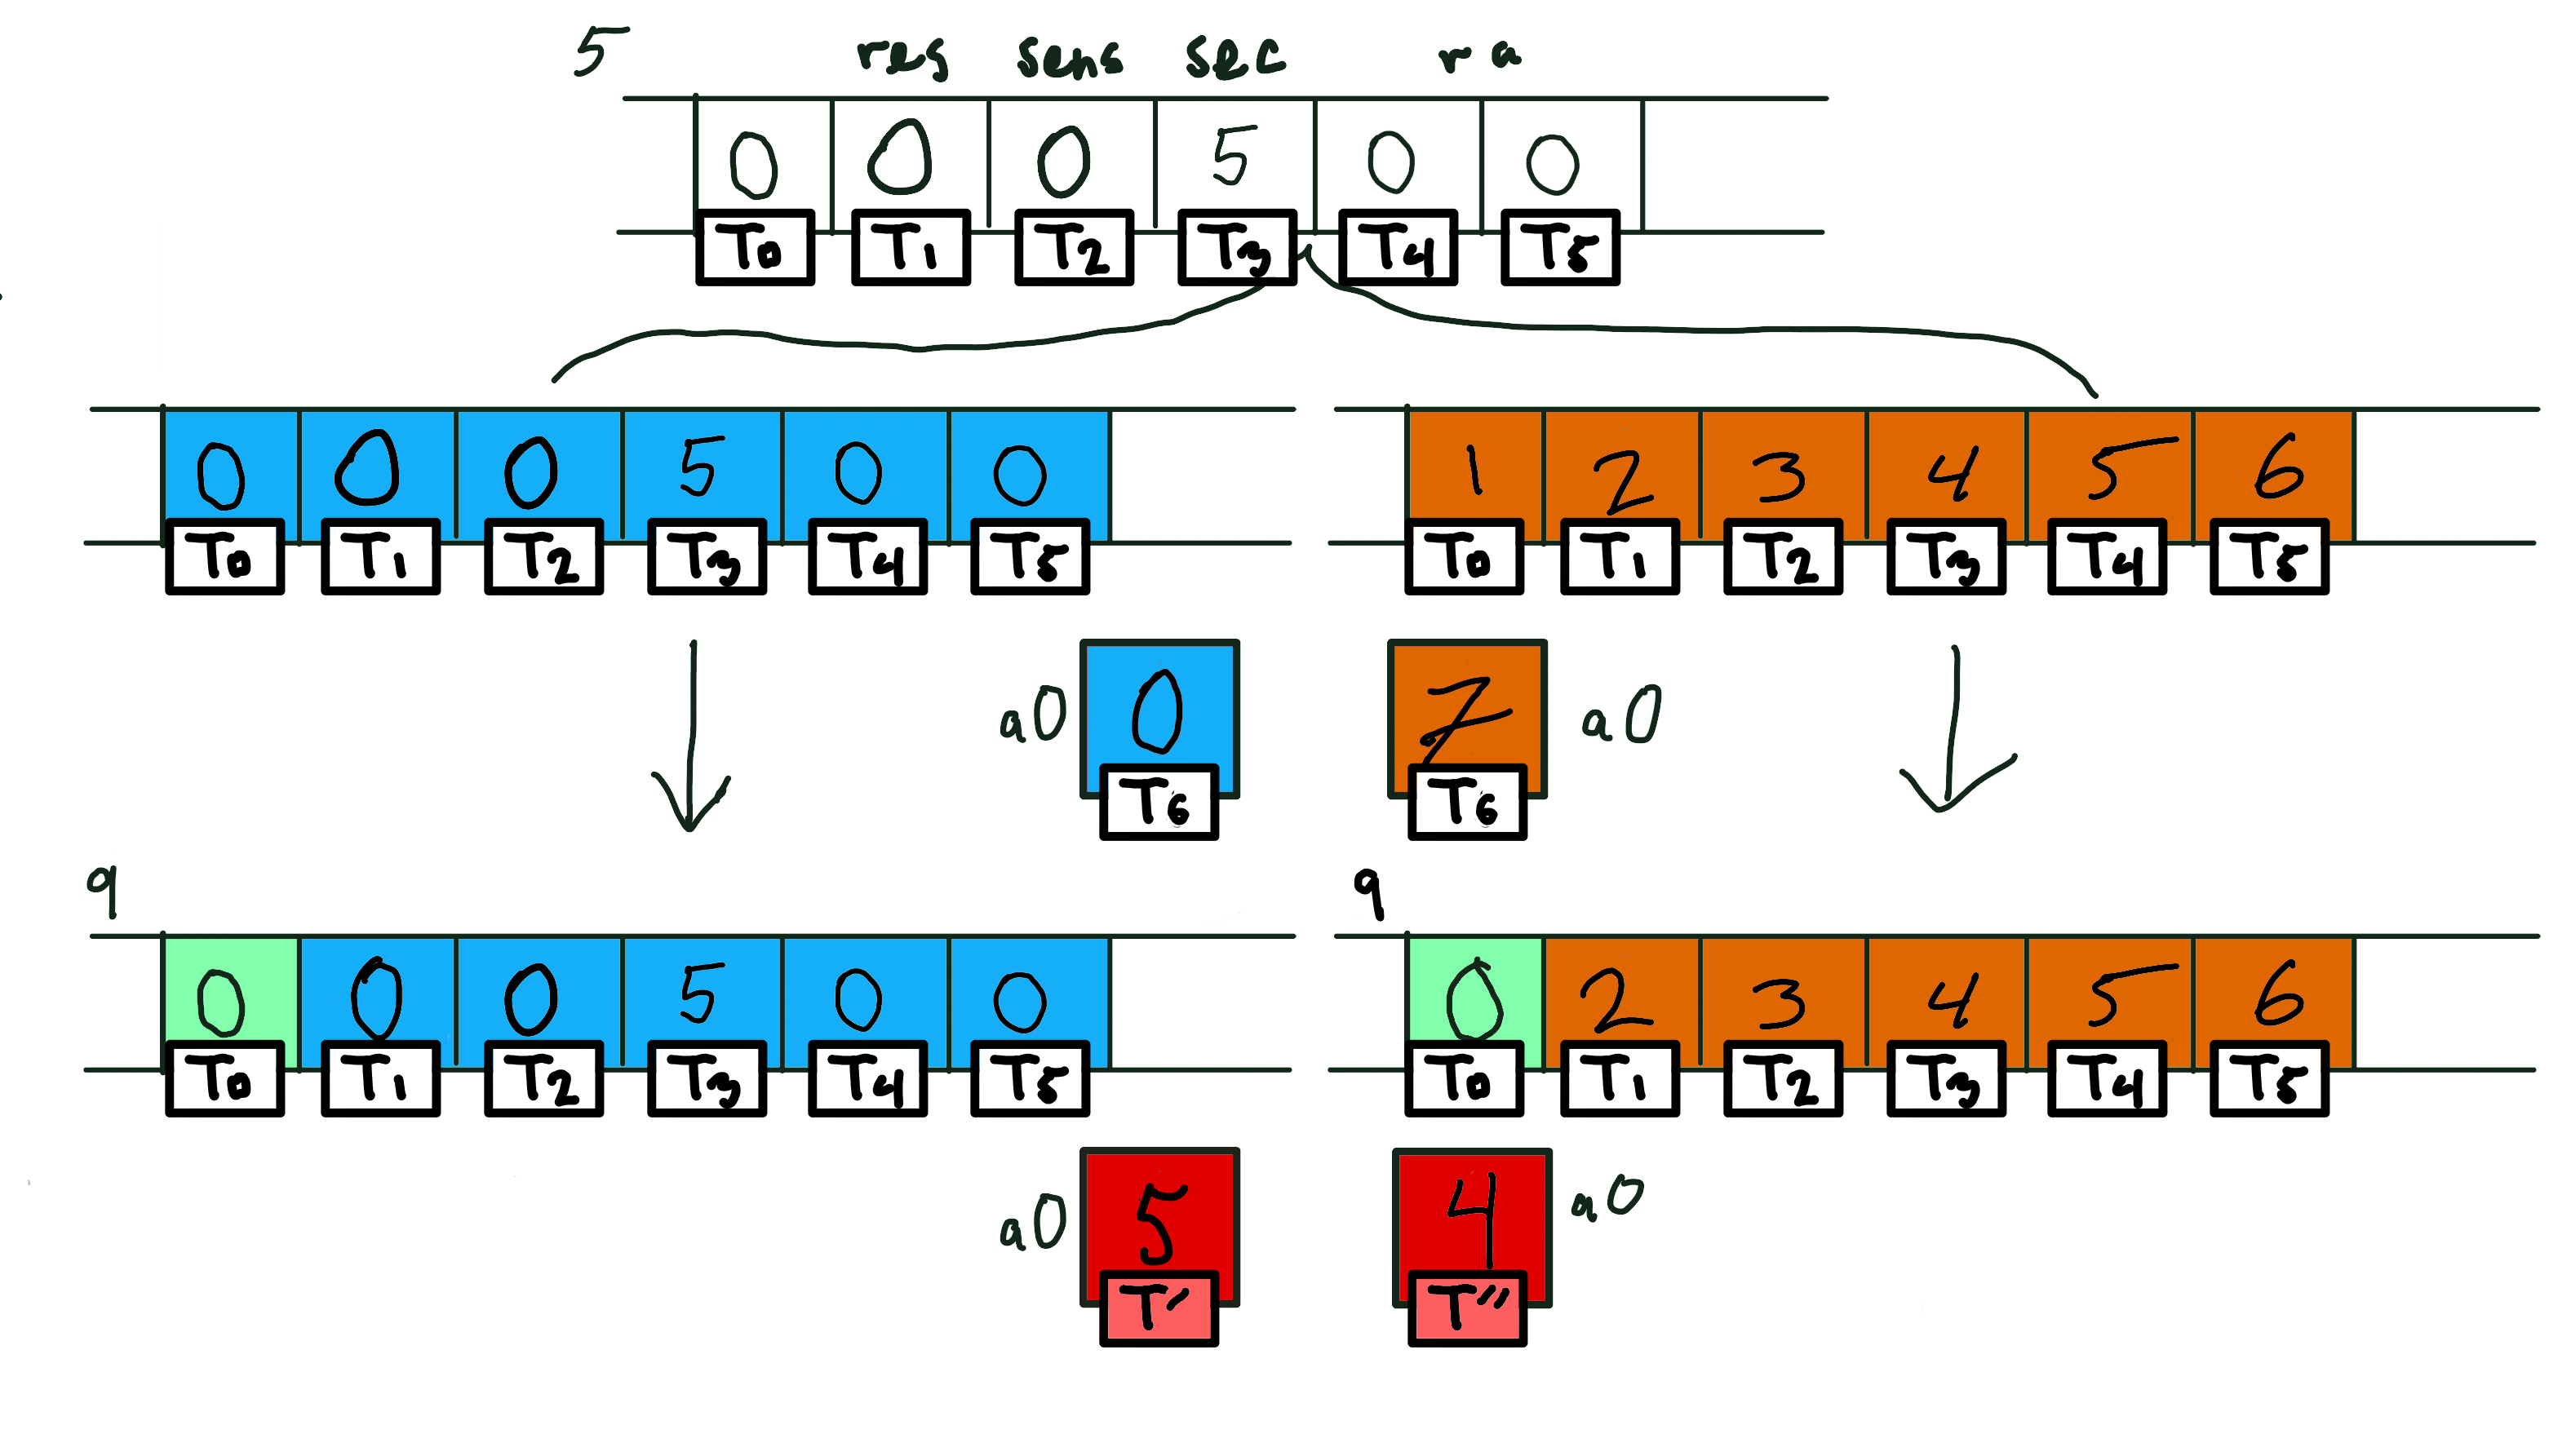
\includegraphics[width=\columnwidth]{variants3.png}
  \caption{Return-time Confidentiality Violation}
  \label{fig:variant3}
\end{figure}
%
Now consider three elements: the address \(\SP - 4\), the address \(\SP + 12\),
and the register {\tt a0}. The execution from the right-hand state to its return
has changed the value at \(\SP - 4\), but that value matches that of the
left-hand return. Therefore, the change does not represent a leak.

The return states disagree on the value of \(\SP + 12\). But in neither
case has that value changed since the original variants. So the difference is inherited from
the original variation, and does not represent a leak either. We do not continue executing the
variant state after return, so these values will not cause the caller to behave differently.

But in the case of {\tt a0}, the value has changed during the call (in both the original
and the variant, although only one of these would be necessary), and its final value
differs between the variants.
Therefore, it must depend on a secret (in fact, the variable {\tt secret}).
Unless {\tt a0} happens to be irrelevant, this is a violation of what
we term {\it return-time confidentiality}.

Structurally, return-time confidentiality resembles integrity, but now dealing with
variants. We begin with a state immediately following
a call, \(\mach\). We consider an arbitrary variant state,
\(\nach\), which may vary any element that is \(\sealed\) or \(\unsealed\), 
i.e., any element that is not used legitimately to pass arguments. Caller confidentiality
therefore can be thought of as the callee's insensitivity to elements in its initial state
that are not part of the caller-callee interface.

In place of a predicate we define \(\conf\) as a binary relation on states, 
which holds on eventual return states \(\mach'\) and \(\nach'\)
iff all relevant elements that changed between \(\mach\) and \(\mach'\) or \(\nach\) and \(\nach'\)
are the same in \(\mach\) and \(\nach\). We then define
return-time confidentiality as holding if \(\conf\) holds on the matching return states
from \(\mach\) and \(\nach\), respectively.

Finally, we define caller confidentiality as the 
combination of internal and return-time confidentiality.
While we have separated the definitions of integrity and confidentiality,
in terms of tag-based enforcement, Depth Isolation and Lazy Tagging and Clearing
both enforce both properties. 

\paragraph*{Callee Confidentiality}

Although we presented our initial example from the perspective of the caller, a callee
may also have data that must be kept secret from its caller. Consider a callee that makes
a privileged system call to obtain a secret key, and uses that key to perform a specific
task. An untrustworthy or erroneous caller might attempt to read the key out of the callee's
memory after return.

We model this as nearly dual to caller integrity: the callee's secrets are those
values that it has stored in \(\unsealed\) elements. So, callee confidentiality means that
at the state following the callee's return, any relevant element that was \(\unsealed\) under
the callee's view retains its original value.

Once again, both tag-based approaches do enforce callee confidentiality, but it is
worth keeping separate because some enforcement mechanisms might not, and it has not
historically been acknowledged by all formal treatments of stack safety \cite{Georges22:TempsDesCerise}.

\paragraph*{The Hierarchy of Stack Safety}

The forms of stack safety described above are largely independent of one another, and
can potentially be enforced separately in various combinations. This is important, because
many existing enforcement mechanisms enforce only some of the stack safety
properties. Stricter enforcement may have greater performance impacts, leading to decisions
about trade-offs between different degrees of stack safety.

In principle, these properties can exist in any combination, but in practice we see examples
of certain combinations that form a hierarchy. Many enforcement techniques focus purely on
well-bracketed control flow. Stack canaries aim to prevent certain attacks on the return
address, and shadow stacks with protection (e.g. Return Address Defender \cite{Chiueh2001RAD})
to enforce it completely.

Others combine this protection with some degree of memory protection,
chiefly focusing on integrity. Skorstengaard et al. \cite{SkorstengaardSTK} characterize stack
safety as the combination of WBCF and {\it local state encapsulation} (LSE), and prove that their
capability-based enforcement satisfies both. LSE corresponds to integrity, plus the
confidentiality of the caller's frame, but not of the unallocated stack or data left
behind in it by previous callees.
They offer a fully abstract overlay semantics, which formalizes WBCF and LSE
together as a safe-by-construction abstract machine. That machine does not allow a callee to
read or write its caller's frame, but might allow it to read data that is left behind below
the caller's frame, which is weaker than our full caller confidentiality and rules out
callee confidentiality entirely. Georges et al. \cite{Georges22:TempsDesCerises} correct
both limitations.

\section{Formalizing Properties}

We have described informally how the security context develops as the system performs
security-relevant operations. Formally, we combine each machine state with a context
to create a {\it combined state} \(s = (\mach,\context)\) and a lift the transition
transition \(\stepstounder{}\) on combined states, labeled with the same operations.
with each step, the context updates based on the function
\(Op : \MACHS \rightarrow \CONTEXTS \rightarrow \psi \rightarrow \CONTEXTS\).
Note that \(Op\) takes as its first argument the state {\it before} the step.
Since a single step might correspond to multiple operations, we apply
\(Op\) as many times as is needed.

\judgmenttwo{\(\mach \xrightarrow{\overline{\psi}} \mach', \obs \)}
            {\(\mathit{foldl} ~ (Op ~ \mach) ~ \context ~ \overline{\psi} = \context'\)}
            {\((\mach,\context) \stepstounder{\overline{\psi}} (\mach', \context', \obs)\)}

The definition of \(Op\) is most convenient to present decomposed into
rules for each operation. In the simple system, the operations affect the
context as follows:

\judgmentbr[Alloc]
           {\(b = \mach[\SP] + \mathit{off}\)}
           {\(V' = V \llbracket \addr \mapsto \sealed |
             b \leq a < b+\mathit{sz} \land V ~ \addr = \unsealed \rrbracket\)}
           {\(Op ~ \mach ~ (\mathbf{alloc} ~ \mathit{off, sz}) ~ (V,\sigma) = (V',\sigma)\)}

\judgmentbr[Call]
           {\(\psi = \mathbf{call} ~ \addr_{target} ~ \overline{\reg_{args}}\)}
           {\(V' = V \llbracket \reg \mapsto \unsealed | \reg \in \mathit{CLR} \rrbracket
             \llbracket \reg \mapsto \public | \reg \in \overline{\reg_{args}} \rrbracket\)}
           {\(Op ~ \mach ~ \psi ~ (V,\sigma) =
             (V',V::\sigma)\)}

\judgment[Ret]
         {\(\sigma = (V,\addr_{ret},\addr_{sp})::\sigma'\)}
         {\(Op ~ \mach ~ \mathbf{return} ~ (\_, \sigma) = (V, \sigma)\)}

            
\subsection{Events and Traces}
\label{sec:events}

We abstract over the events that can be observed in the system, defining them
only as a set \(\OBSS\) that contains at least the element \(\tau\), the silent
event. Other events might represent certain function calls (i.e., system calls)
or writes to special addresses representing mmapped regions.
A {\em trace} is a nonempty, finite or infinite sequence
of events, ranged over by \(\obsT\).
We use ``\(\notfinished{}{}\)'' to represent ``cons'' for traces, reserving ``::''
for list-cons.

We write that execution from a state produces an observation trace
\(\mach,\context \hookrightarrow \obsT\) as follows, coinductively:

\judgmenttwo{\((\mach,\context) \stepstounder{} (\mach',\context',\obs)\)}
            {\((\mach',\context') \hookrightarrow \obsT\)}
            {\((\mach,\context) \hookrightarrow \notfinished{\obs}{\obsT}\)}

We define another relation that takes a trace until we have returned from the
active principal.
We write this \(d \downarrow (\mach,\context) \hookrightarrow \obsT\), where
\(d\) is the depth of the current call.

\judgment{\(|\sigma| < d\)}
         {\(d \downarrow (\mach,(V,\sigma)) \hookrightarrow \tau\)}

\judgmenttwobrlong{\((\mach,(V,\sigma)) \stepstounder{} (\mach',\context',\obs)\)}
                  {\(|\sigma| \geq d\)}
                  {\(d \downarrow (\mach',\context') \hookrightarrow \obsT\)}
                  {\(d \downarrow (\mach,(V,\sigma)) \hookrightarrow \notfinished{\obs}{\obsT}\)}

\paragraph*{Observational Similarity}

We say that two event traces $\obsT_1$ and $\obsT_2$ are {\em similar},
written \(\obsT_1 \eqsim \obsT_2\), if the sequence of non-silent events
is the same. That is, we compare up to deletion of \(\tau\) events.

\begin{minipage}{.4\columnwidth}
  \judgment{}{\(\obsT \eqsim \obsT\)}
\end{minipage}
\begin{minipage}{.4\columnwidth}
  \judgment{\(\obsT_1 \eqsim \obsT_2\)}
           {\(\notfinished{\obs}{\obsT_1} \eqsim \notfinished{\obs}{\obsT_2}\)}
\end{minipage}

\begin{minipage}{.4\columnwidth}
  \judgment{\(\obsT_1 \eqsim \obsT_2\)}
           {\(\notfinished{\tau}{\obsT_1} \eqsim \obsT_2\)}
\end{minipage}
\begin{minipage}{.4\columnwidth}
  \judgment{\(\obsT_1 \eqsim \obsT_2\)}
           {\(\obsT_1 \eqsim \notfinished{\tau}{\obsT_2}\)}
\end{minipage}

\paragraph*{Variants and Irrelevant Values}

For a given system, assume an equivalence class \(\sim\) on values.
Two states are variants with respect to a set of elements, \(\components\),
if they agree on the value of every element not in \(\components\) and
all of their values are equivalent under \(\sim\).
Our notion of non-interference involves comparing the traces of such
\(\components\)-variants. We use this to define sets of irrelevant elements,
and secrets in general.

\definition Machine states \(\mach\) and \(\nach\) are {\em \(\components\)-variants},
written \(\mach \approx_\components \nach\), if, for
all \(\component \not \in \components\), \(\mach[\component] = \nach[\component]\)
and for all \(\component\), \(\mach[\component] \sim \nach[\component]\).

\definition An element set \(\components\) in state \((\mach,\context)\) contains
irrelevant values, written \((\mach,\context) \parallel \components\), if for all
\(\nach\) such that \(\mach \approx_{\components} \nach\), if 
\((\mach,\context) \hookrightarrow \obsT\) and
\((\nach,\context) \hookrightarrow \obsT'\), then
\(\obsT \eqsim \obsT'\).

\subsection{Facts Abouts Calls and Returns}
\label{sec:facts}

Here we define some logical operations to reason about the behavior of the
system over time. These have a temporal-logic flavor, as they reflect
the expected behavior of the system in the future, after a possible return.

\paragraph*{On-return}

The intuition behind integrity (below) is that a caller may expect its
sealed data to be unchanged when control returns to it. In fact, the callee
may overwrite such data---when the data are found in callee-saved registers
this is perfectly legal---as long as it either restores it, or has some guarantee
that its changes will not impact the caller.

We start by defining a second-order logical operator
\(d \uparrow P\), pronounced ``\(P\) holds on return from depth \(d\),''
where \(P\) is a predicate on machine states. This is a coinductive relation
similar to ``weak until'' in temporal logic---it also holds if the program never
returns from depth \(d\).

\judgmenttwo[Returned]
            {\(|\sigma| < d\)}
            {\(P ~ (\mach,(V,\sigma))\)}
            {\((d \uparrow P) ~ (\mach, (V,\sigma))\)}

\judgmenttwobrlong[Step]
                  {\(|\sigma| \geq d\)}
                  {\((d \uparrow P) ~ (\mach', \context')\)}
                  {\((\mach, (V,\sigma)) \stepstounder{\overline{\psi}} (\mach', \context',\obs)\)}
                  {\((d \uparrow P) ~ (\mach, (V,\sigma))\)}

Similarly, for confidentiality, we will want to compare pairs of future states,
so we give a binary equivalent, \(d \Uparrow R\), where
\((\mach,\context) ~ (d \Uparrow R) ~ (\mach',\context')\) holds if \(R\) holds on the
first states that return from depth \(d\) after \((\mach,\context)\) and \((\mach',\context')\),
respectively. Once again, \(\Uparrow\) is coinductive.

\judgmenttwobrlong[Returned]
            {\(|\sigma_1| < d\)}
            {\(|\sigma_2| < d\)}
            {\((\mach_1,(V_1,\sigma_1)) ~ R ~ (\mach_2,(V_2,\sigma_2))\)}
            {\((\mach_1,(V_1,\sigma_1)) ~ (d \Uparrow R) ~ (\mach_2,(V_2,\sigma_2))\)}

\judgmenttwobrlong[Left]
              {\(|\sigma_1| \geq d\)}
              {\((\mach_1,(V_1,\sigma_1)) \stepstounder{\overline{\psi}} (\mach_1',\context_1',\obs)\)}
              {\((\mach_1',\context_1') ~ (d \Uparrow R) ~ (\mach_2,(V_2,\sigma_2))\)}
              {\((\mach_1,(V_1,\sigma_1)) ~ (d \Uparrow R) ~ (\mach_2,(V_2,\sigma_2))\)}

\judgmenttwobrlong[Right]
              {\(|\sigma_2| \geq d\)}
              {\((\mach_2,(V_2,\sigma_2)) \stepstounder{\overline{\psi}} (\mach_2',\context_2',\obs)\)}
              {\((\mach_1,(V_1,\sigma_1)) ~ (d \Uparrow R) ~ (\mach_2,\context_2')\)}
              {\((\mach_1,(V_1,\sigma_1)) ~ (d \Uparrow R) ~ (\mach_2,(V_2,\sigma_2))\)}

\subsection{Properties}
\label{sec:props}

\paragraph*{Well-bracketed Control Flow}

\definition We define a correct return from \(\mach\) as:
%
\[\ret(\mach) = \{(\mach',\context') \mid \mach'[\SP] = \mach[\SP] \land \mach'[\PCname] = \mach[\PCname]+4\}\]

\definition
A system enjoys  well-bracketed control flow if, whenever
\((\mach,\context) \stepstounder{\overline{\psi}} (\mach',(V,\sigma),\obs)\) where 
\(\mathbf{call} ~ \addr ~ \overline{\reg} \in \bar{\psi}\),
\(|\sigma| \uparrow \ret(\mach)\) holds on \((\mach',(V,\sigma))\).

\paragraph*{Integrity}

\definition Let \(\Delta(\mach,\mach')\) be the set of elements \(\component\)
such that \(\mach[\component] \not = \mach'[\component]\).

\definition We define \(\intProp(\mach,V)\), to hold on a state \((\mach',\context')\) when
\(\{\component \mid V ~ \component = \sealed\} \cap \Delta(\mach,\mach')\)
is irrelevant in \((\mach', \context')\).

\definition A system enjoys {\it stack integrity} if, whenever
\((\mach,\context) \stepstounder{\overline{\psi}} (\mach',(V,\sigma),\obs)\) with
\(\mathbf{call} ~ \addr ~ \overline{\reg} ~ \overline{sa} \in \bar{\psi}\),
we have:
\[(|\sigma'| \uparrow \intProp(\mach',V)) ~ (\mach',(V,\sigma))\]

\paragraph*{Caller Confidentiality}

\definition Let \((\mach,\context)\) be a state with \(\context = (V,\sigma)\), and
\(\components = \{\component \mid V ~ \component \in \{\sealed, \unsealed\}\}\).
Then \((\mach,\context)\) enjoys {\it internal confidentiality} with respect to \(\components\)
if, for any \(\nach\) that is a \(\components\)-variant of \(\mach\), we can take
\(|\sigma| \uparrow (\mach,\context) \hookrightarrow \obsT\) and
\(|\sigma| \uparrow (\nach,\context) \hookrightarrow \obsT'\) and have that
\(\obsT \simeq \obsT'\).

\definition The {\em corrupted set} \(\bar{\Diamond}(\mach,\mach',\nach,\nach')\)
is the set \((\Delta(\mach,\mach') \cup \Delta(\nach,\nach')) \cap \Delta(\mach',\nach')\).
This treats
\(\mach\) and \(\nach\) as the initial states and
\(\mach'\) and \(\nach'\) as their corresponding final states, and is the
set of elements that were corrupted between them.

\definition We define the relation \(\conf(\mach,\nach)\) to hold on a pair of states
\((\mach',\context)\) and \((\nach',\context')\) when
\(\bar{\Diamond}(\mach,\nach,\mach',\nach')\) is irrelevant in \((\mach',\context)\).

\definition A state \((\mach,(V,\sigma))\) enjoys {\it return-time confidentiality}
if, for \(\components = \{\component \mid V ~ \component \in \{\sealed, \unsealed\}\}\)
and any \(\nach\) that is a \(\components\)-variant of \(\mach\), we have:
\[(\mach,(V,\sigma)) ~ (|\sigma| \Uparrow \conf(\mach,\nach) ~ (\nach,(V,\sigma))\]

\definition A system enjoys {\it caller confidentiality} if, whenever
\((\mach,\context) \stepstounder{\overline{\psi}} (\mach',\context',\obs)\)
with \(\mathbf{call} ~ \addr ~ \overline{\reg} ~ \overline{sa} \in \psi\),
\((\mach',\context')\) enjoys both internal and return-time confidentiality.

\paragraph*{Callee Confidentiality}

\definition We define \(\cconf(\mach,V)\), to hold on a state \((\mach',\context')\) when
\(\{\component \mid V ~ \component = \unsealed\} \cap \Delta(\mach,\mach')\)
is irrelevant in \((\mach', \context')\).

\definition A system enjoys {\it callee confidentiality} if, whenever
\((\mach,\context) \stepstounder{\overline{\psi}} (\mach',(V,\sigma),\obs)\)
with \(\mathbf{call} ~ \addr ~ \overline{\reg} ~ \overline{sa} \in \psi\),
% or \(\mathbf{tailcall} ~ \addr ~ \overline{\reg} ~ \overline{sa} \in \psi\),
we have:
\[(|\sigma| \uparrow \cconf(\mach',V)) ~ (\mach',\context')\]

\section{Advanced Machine}

The advanced machine defines additional operations, and extends some of the old ones.
It adds a field \(\overline{sa}\) to the \(\mathbf{call}\) operation, which is a set of
triples of a register, a base offset, and a size, and denotes that the object at the offset
from the given register is to be passed as an argument. The new \(\mathbf{tailcall}\) operation
has the same fields, but deals with tail call optimizations in which the callee will reuse
the caller's stack. The \(\mathbf{alloc}\) operation
gains a boolen flag indicating whether the allocation is to be public, accessible to
all functions until deallocated. And, we add the corresponding \(\mathbf{dealloc}\)
operation.

\begin{align*}
  \psi \in \Psi ::= & \mathbf{call} ~ \addr_{target} ~ \overline{\reg_{args}} ~ \overline{sa} &
  sa \in \REGS \times \mathbb{Z} \times \mathbb{N} \\
  | & \mathbf{tailcall} ~ \addr_{target}  ~ \overline{\reg_{args}} ~ \overline{sa} &
  sa \in \REGS \times \mathbb{Z} \times \mathbb{N} \\
  | & \mathbf{return} & \\
  | & \mathbf{alloc} ~ \mathit{pub} ~ \mathit{off ~ sz} & \mathit{off, sz} \in \mathbb{N}, \mathit{pub} \in \mathbb{B} \\
  | & \mathbf{dealloc} ~ \mathit{off ~ sz} & \mathit{off, sz} \in \mathbb{N} \\
\end{align*}

\subsection{Public Allocations}

The advanced machine supports public stack allocations that can
be accessed by anyone until they are deallocated on their owner's return,
represented by \(\mathbf{alloc} ~ \mathbf{t} \dots\).
For example, consider the following code:

{\tt
  void g() \{

  ~ ~ int x[3];

  ~ ~ int y;

  ~ ~ h(\&x);
    
  \}
}

Here we have allocated several arrays and variables; {\tt y}
will behave as normal with \(\mathbf{alloc} ~ \mathbf{f} \dots\), but
{\tt x} has its address taken and passed to another function. That
function might do anything at all to {\tt x}, and might store its pointer
elsewhere (in the heap, for instance) so that the scope of legitimate accesses
to {\tt x} are uncertain. We default to assuming that any address-taken local
should be public. Meanwhile {\tt y} is still private.

In the likely event that the space for the return address, {\tt x}, and {\tt y}
are all allocated in a single step, that step makes multiple allocation operations:
\[\bar{\psi} = [\mathbf{alloc} ~ \mathbf{f} ~ (-20,4);
 \mathbf{alloc} ~ \mathbf{t} ~ (-16,12) ; \mathbf{alloc} ~ \mathbf{f} ~ (-4,4)]\]

Allocating public objects affects the call stack very similarly to private ones,
but instead of labeling them \(\object\) they become \(\public\), so they are
not sealed at a call. This makes these
regions of memory able to transmit information between caller and callee without
violating the stack safety properties. Note that there is no way to seal a location
once it has become \(\public\); only when {\tt x} is deallocated will its region
be available to allocate privately.

\judgmentbr[AllocPriv]
           {\(b = \mach[\SP] + \mathit{off}\)}
           {\(V' = V \llbracket \addr \mapsto \sealed |
             b \leq a < b+\mathit{sz} \land V ~ \addr = \unsealed \rrbracket\)}
           {\(Op ~ \mach ~ (\mathbf{alloc} ~ \mathbf{f} ~ \mathit{off, sz}) ~ (V,\sigma) = (V',\sigma)\)}

\judgmentbr[AllocPub]
           {\(b = \mach[\SP] + \mathit{off}\)}
           {\(V' = V \llbracket \addr \mapsto \public |
             b \leq a < b+\mathit{sz} \land V ~ \addr = \unsealed \rrbracket\)}
           {\(Op ~ \mach ~ (\mathbf{alloc} ~ \mathbf{t} ~ \mathit{off, sz}) ~ (V,\sigma) = (V',\sigma)\)}

\judgmentbr[Dealloc]
           {\(b = \mach[\SP] + \mathit{off}\)}
           {\(V' = V \llbracket \addr \mapsto \unsealed |
             b \leq a < b+\mathit{sz} \land V ~ \addr \in \{\object, \public\} \rrbracket\)}
           {\(Op ~ \mach ~ (\mathbf{dealloc} ~ \mathit{off, sz}) ~ (V,\sigma) = (V',\sigma)\)}

\subsection{Stack Arguments}

So far, we have not dealt with arguments spilled onto the stack, variadic arguments,
or arguments that are passed by reference without their addresses being taken
explicitly (i.e., structs and arrays passed directly.) Consider the simplest case,
where a function has more than 8 arguments and therefore must (in RISC-V) spill one
to the stack.

{\tt
  void main() \{

  ~ f(1,2,3,4,5,6,7,8,9);

  ~ g(42);
  
  \}
}

\vspace{\abovedisplayskip}

\begin{tabular}{r l | l}
  \labeledrow{0:}{addi sp,sp,-12}{\(\mathbf{alloc} ~ (-12,12)\)}
  \labeledrow{4:}{sd ra,4(sp)}{}
  \labeledrow{8:}{li a5,9}{}
  \labeledrow{12:}{sd a5,0(sp)}{}
  \labeledrow{16:}{li a7,8}{}
  \dots \\
  \labeledrow{48:}{jal 100,ra}{\(\mathbf{call} ~ \{\mathtt{a0-a7}\} ~ \{(\SP,0,4)\}\)}
  \labeledrow{52:}{li a0,42}{}
  \labeledrow{56:}{jal 200,ra}{\(\mathbf{call} ~ \{\mathtt{a0}\} ~ \emplist\)}
  \dots \\
\end{tabular}

Under a typical calling convention, the callee expects the ninth argument to
be passed to it at bottom of the caller's frame, so the caller allocates extra
space for it. Then the call to {\tt f} identifies that we expect a range of four
bytes from the stack pointer to be passed as an object instead of sealed.

So we must refine our call operation to make use of the information that we have about
which memory contain arguments, \(\overline{sa}\). \(\overline{sa}\) is a set of
triples of a register, an offset from the value of that register, and a size.
We first define the helpful set \(\mathit{passed} ~ \overline{sa} ~ \mach\),
then extend the call operation to keep all objects in \(\mathit{passed}\) marked
as \(\object\) and seal everything else.
%
\[\mathit{passed} ~ \overline{sa} ~ \mach \triangleq
\bigcup_{(\reg,b,o) \in \overline{sa}} \{\mach[\reg]+i | b \leq i < b+o\}\]
%
\judgmentbrbr[]
             {\(\psi = \mathbf{call} ~ \addr_{target} ~ \overline{\reg_{args}} ~ \overline{sa}\)}
             {\(V' = V \llbracket \reg \mapsto \unsealed | \reg \in \mathit{CLR} \rrbracket
               \llbracket \reg \mapsto \public | \reg \in \overline{\reg_{args}} \rrbracket\)}
             {\(V'' = V'\llbracket \addr \mapsto \sealed | V' ~ \addr = \object \land \addr \not \in (\mathit{passed} ~ \overline{sa} ~ \mach) \rrbracket\)}
             {\(Op ~ \mach ~ \psi ~ (V,\sigma) =
               (V'',V::\sigma)\)}

The remaining definitions are unchanged. Now a stack-spilled argument can be allocated
and remain accessible in the callee, while its memory is sealed for calls that do not
use that memory as an argument.

This same structure works for pass-by-reference arguments. In this case {\tt main}
passes an array {\tt x} directly, which is compiled as a pass-by-reference.

{\tt
  int main() \{
  
  ~ int x[1];

  ~ f(x);

  ~ g();

  ~ return x[0];

  \}
}

Unlike the address-taken array, we can clearly delineate the scope in which {\tt x} may be
accessed without violating stack safety: {\tt f} should be allowed to access it, but further
calls from {\tt f} should not (unless {\tt f} passes it to them) and {\tt g} certainly
should not. Say the compiler opts to pass the pointer to {\tt x} in register {\tt a0}.
The {\tt f} is specifically being given access to the four bytes starting at that address.
The call operation is \(\mathbf{call} ~ \emplist ~ \{(\mathtt{a0},0,4)\}\).

\subsection{Tail Calls}

The operation rule for a tailcall is similar to that for a normal call.
We do not push the caller's view onto the stack,
but replace it outright. This means that a tailcall does not increase the size of
the call stack, and therefore for purposes of our properties, all tailcalls will
be considered to return simultaneously when the eventual {\bf return} operation
pops the top of the stack.

Since the caller will not be returned to, it does not need integrity, though
it should still enjoy confidentiality. We set its frame to \(\unsealed\) rather
than \(\sealed\) to express this. Of course, some objects may be passed in place,
easily modeled by including them in \(\overline{sa}\).

\judgmentbrbr[]
             {\(\psi = \mathbf{call} ~ \addr_{target} ~ \overline{\reg_{args}} ~ \overline{sa}\)}
             {\(V' = V \llbracket \reg \mapsto \unsealed | \reg \in \mathit{CLR} \rrbracket
               \llbracket \reg \mapsto \public | \reg \in \overline{\reg_{args}} \rrbracket\)}
             {\(V'' = V'\llbracket \addr \mapsto \unsealed | V' ~ \addr = \object \land \addr \not \in (\mathit{passed} ~ \overline{sa} ~ \mach) \rrbracket\)}
             {\(Op ~ \mach ~ \psi ~ (V,\sigma) =
               (V',\sigma)\)}
             
\subsection{Provenance, Capabilities, and Protecting Objects}

What if we want to express a finer-grained notion of safety, in which
stack objects are protected unless the function that owns them intentionally
passes a pointer to them? This can be thought of as a {\it capability}-based
notion of security. Capabilities are unforgeable tokens that grant access to
a region of memory, typically corresponding to valid pointers to that region.
So, in order to express such a property, we need our machine to carry some notion
of {\it pointer provenance}---a distinction between a pointer that is intended to
point to a given object, and non-pointer integers as well as pointers to other objects.

One such provenance model is Memarian et al.'s PVI \cite{}, in which pointers are
annotated with the identity of the object they first pointed to. This annotation is
propagated when the pointer is copied and when operations are performed on it---even
integer-only operations.

We can model this as a pair of additional security-relevant operations: one which
declares a register to contain a valid pointer, and one which transmits the provenance
of a pointer from one element to another.

\begin{align*}
  \psi \in \Psi ::= & \dots \\
  & \mathbf{promote} ~ \reg ~ sa & sa \in \REGS \times \mathbb{Z} \times \mathbb{N} \\
  & \mathbf{propagate} ~ \component_{src} ~ \component_{dst} \\
\end{align*}

In addition to the normal call stack, our security context will carry a map \(\rho\) from
elements to memory regions, represented as a base and a bound \(\context = (V, \sigma, \rho)\).
Existing operations are extended to keep the value of \(\rho\) the same, and the new operations
work as follows:

\judgmenttwobrlong[]
                  {\(\psi = \mathbf{promote} ~ \reg_{dst} ~ (\reg_{base},\mathit{off},sz)\)}
                  {\(b = \mach[\reg_{base}]+\mathit{off}\)}
                  {\(\rho' = \rho[\reg \mapsto (b,b+sz)]\)}
                  {\(Op ~ \mach ~ \psi ~ (V,\sigma,\rho) = (V,\sigma,\rho')\)}

\judgmenttwo[]
            {\(\psi = \mathbf{propagate} ~ \component_{src} ~ \component_{dst}\)}
            {\(\rho' = \rho[\component_{dst} \mapsto \rho[\component_{src}]]\)}
            {\(Op ~ \mach ~ \psi ~ (V,\sigma,\rho) = (V,\sigma,\rho')\)}

We now have a notion of provenance, and must integrate it into the definition of
stack safety. We essentially generalize the above notion of passing: we will consider
a caller to have intentionally passed an object if that object is reachable by
a capability that has been passed to the callee. This includes capabilities passed
indirectly, by being stored in an object that is in turn passed. Formally, we call
this set \(\mathit{capped}\), and define it recursively:

\[\begin{split}
& \mathit{capped} ~ \components ~ \rho \triangleq \bigcup_{\component \in \components} \{\component\} \cup \mathit{capped} ~ \components' ~ \rho \textnormal{ where} \\
& \components' = \{\component' |\rho[\component] = (\mathit{base},\mathit{bound})
\land \mathit{base} \leq \component' < \mathit{bound}\} \\
\end{split}\]

We then tweak the call operation to seal only objects that are in \(\mathit{capped}\), or
the previously defined \(\mathit{passed}\).

\judgmentbrbrbr[]
               {\(\psi = \mathbf{call} ~ \addr_{target} ~ \overline{\reg_{args}} ~ \overline{sa}\)}
               {\(V' = V \llbracket \reg \mapsto \unsealed | \reg \in \mathit{CLR} \rrbracket
                 \llbracket \reg \mapsto \public | \reg \in \overline{\reg_{args}} \rrbracket\)}
               {\(\components = \{\addr | V' ~ \addr = \object \land \addr \not \in (\mathit{passed} ~ \overline{sa} ~ \mach) \cup (\mathit{capped} ~ \overline{\reg_{args}} ~ \rho) \}\)}
               {\(V'' = V'\llbracket \components \mapsto \sealed \rrbracket\)}
               {\(Op ~ \mach ~ \psi ~ (V,\sigma,\rho) =
                 (V'',V::\sigma,\rho)\)}

Note that we have a degree of monotonicity here. Once an object is sealed (because its
capability has not been passed to a callee), subsequent nested calls can never unseal it.
On the other hand, an object that is passed via a pointer may be passed on indefinitely.

%\section{Enforcement}
%\label{sec:enforcement}

%We use our properties to test the stack safety micro-policies of Roessler and DeHon,
%particularly their Lazy Tagging and Clearing. Our underlying machine is a RISC-V
%based on the MIT RISC-V formalism \cite{} and extended with {\it metadata tags},
%represented as additional state in \(\mathcal{P}\), one for each register, address,
%and the program counter:
%\[\mathcal{P} ::= t_\reg | t_\addr | t_\PCname\]
%
%We divide values into normal memory words and tags drawn from a policy-specific
%set of tags \(\mathcal{T}\), \(\mathcal{V} ::= \mathcal{W} | \mathcal{T}\).
%The machine's step function corresponds to that of the basic RISC-V machine,
%with the behavior of the tags at each step parameterized by a {\it micro-policy},
%which may turn a normal step into an error (represented by returning to the same state.)

%\paragraph*{Protecting Enforcement State}

%State beyond registers and memory is always considered \(\public\), and in a PIPE machine this
%includes tags. That does not mean that functions should be modifying them! It just means that we
%do not consider them to be part of the state being protected. It is less obvious that a function
%should be prevented reading a tag, and our properties do not rule it out, although in practice
%PIPE does not allow such reads. It would be quite possible to implement
%the properties so that they would forbid these activities, for instance by structuring \(\mathcal{P}\)
%to treat tags separately and apply stack safety to the tags on the stack, but there is no obvious
%application for such a stringent property---the enforcement state must be protected in order that
%enforcement not be subverted, not for its own sake.

\section*{[Meta] Remainder}

These document sections lay out a way to present our stack safety properties to build intuition and
then introduce the formalism. Next the full paper will need the testing section and an expanded
enforcement section, but these can largely be borrowed from previous submissions.

\bibliographystyle{IEEEtran}
\bibliography{bcp.bib,local.bib}

\end{document}
